\documentclass[12pt, twoside]{book}
\usepackage[a4paper,width=150mm,top=25mm,bottom=25mm,bindingoffset=6mm]{geometry}
\usepackage[utf8]{inputenc}
\usepackage[italian]{babel}
\usepackage{caption}
\usepackage{fancyhdr}
\usepackage{newlfont}
\usepackage{float}
\usepackage{xcolor}
\usepackage[nottoc]{tocbibind}
\usepackage{emptypage}
\usepackage{titlesec}
\usepackage[T1]{fontenc}
\usepackage{blindtext, array}
\usepackage[sorting=none,backend=bibtex]{biblatex}
\usepackage{csquotes}
\usepackage{pdfpages}
\usepackage{listings}
\usepackage{amsmath}
\usepackage[cache=false]{minted}
\usepackage{setspace}
\usepackage[hidelinks]{hyperref}
\usepackage{outline}
\usepackage{enumitem}
\usepackage{mathtools}
\usepackage{xparse}
\usepackage{svg}
\usepackage{tikz}
\usepackage{lipsum}
\usepackage[toc,page]{appendix}
\usepackage{amsfonts}
\usepackage{subcaption}
\usepackage[htt]{hyphenat}
\usetikzlibrary{shapes.geometric, arrows, positioning}


%%%%%%%%%%%%%%%%%%%%%%%%%%%%%%%%%%%%%%%%%%%%%%%
\setlist{nosep}

% Stile di pagina
% \pagestyle{fancy}
\usemintedstyle{colorful}

\definecolor{lightgray}{gray}{0.95}

% Stile dei titoli dei capitoli
\definecolor{gray75}{gray}{0.75}
\newcommand{\hsp}{\hspace{20pt}}
\titleformat{\chapter}[hang]
{\Huge\bfseries}
{\thechapter\hsp\textcolor{gray75}{|}\hsp}
{0pt}
{\Huge\bfseries}

% lnorm command
\DeclarePairedDelimiter{\norm}{\lVert}{\rVert}

\newenvironment{equationderivation}[1][]{%
    \begin{trivlist}%
    \item[]\textbf{Passaggi #1:}%
}{%
    \end{trivlist}%
}

\newenvironment{proof}[1][]{%
    \begin{trivlist}%
    \item[]\textbf{Dimostrazione #1:}%
}{%
    \end{trivlist}%
}

% \raggedbottom
%%%%%%%%%%%%%%%%%%%%%%%%%%%%%%%%%%%%%%%%%%%%%%%

% Bibliografia
\addbibresource{bibliografia.bib}

\onehalfspacing
\begin{document}

\begin{titlepage}
    \begin{center}
        {{\Large{\textsc{Alma Mater Studiorum $\cdot$ Universit\`a di Bologna}}}}
        \rule[0.1cm]{15cm}{0.1mm}
        \rule[0.5cm]{15cm}{0.6mm}
        \\\vspace{3mm}
        {\small{\bf Scuola di Ingegneria e Architettura \\
                Dipartimento di Informatica $\cdot$ Scienza e Ingegneria $\cdot$ DISI\\
                Corso di Laurea Magistrale in Ingegneria Informatica}}
    \end{center}

    \vspace{23mm}

    \begin{center}{
            \large \bf DIFFERENTIAL PRIVACY\par
        }\end{center}
    \vspace{40mm} \par \noindent
    \begin{minipage}[t]{0.47\textwidth}{
        \large{Relatore:
        \vspace{2mm}\\
        {\bf Prof. Michele Colajanni}
        }
        \vspace{4mm}\\
        \large{Correlatore:
        \vspace{2mm}\\
        {\bf Ing. Silvio Russo}
        }
    }
    \end{minipage}
    %
    \hfill
    %
    \begin{minipage}[t]{0.47\textwidth}\raggedleft{
            {\large{Presentata da:
                        \vspace{2mm}\\
                        \bf Riccardo Barbieri}}}
    \end{minipage}
    \vspace{40mm}
    \begin{center}
        Anno Accademico 2023/2024
    \end{center}
\end{titlepage}

\phantomsection
\listoffigures

\tableofcontents

\chapter*{Introduzione}
---\textit{Ancora un placeholder, da modificare}---
La privacy dei dati è diventata una preoccupazione sempre più importante nell'era digitale. Con la crescente raccolta e l'analisi di dati personali, è fondamentale garantire che le informazioni individuali siano protette da accessi non autorizzati e da usi impropri. La privacy differenziale (DP) è una rigorosa definizione matematica di privacy che offre forti garanzie di riservatezza anche quando i dati vengono utilizzati per l'analisi.


\chapter{Stato dell'arte}
\section{Introduzione alla Differential Privacy}
La privacy differenziale (DP) è un framework per la progettazione di algoritmi utilizzati per la creazione di distribuzioni di dati aggregati su dataset; gli algoritmi che rispettano la definizione di DP sono in grado di limitare l'impatto che la partecipazione di un singolo individuo ha sui risultati dell'analisi, rendendo \textit{quasi} impossibile confermare o negare la presenza di un soggetto all'interno del dataset utilizzato per l'aggregazione di dati.

%TODO: espandi sul concetto di quasi impossibile, definire meglio in sezione su promesse differential privacy

Questo risultato è ottenuto grazie all'aggiunta di rumore casuale campionato da una distribuzione di probabilità opportuna ai risultati dell'elaborazione dei dati.

Lo scopo principale degli algoritmi DP è quello di poter garantire ai partecipanti di un dataset che la privacy dei dati forniti non potrà essere violata a seguito di analisi effettuate sul dataset, indipendentemente dalla disponibilità di altre fonti di informazioni su uno specifico individuo \cite[p.~5]{TCS-042}.

\subsection{Definizione}
La definizione seguente costituisce un formalismo più ristretto rispetto alla definizione completa, quest'ultima include un secondo parametro $\mathcal{\delta}$, la cui funzione e utilità verranno discusse in seguito.

Una trasformazione $\mathcal{M}$ è considerata $\varepsilon$-differenzialmente privata se, per ogni dataset $D_1$ e $D_2$ che differiscono al massimo per un individuo ($\norm{D_1 - D_2}_1 \le 1$) e ogni $S \subseteq \operatorname{Range}(\mathcal{M})$, vale la seguente disequazione \cite{10.1007/11681878_14}:
\begin{equation}
  \Pr[\mathcal{M}(D_1) = S] \le e^{\varepsilon} \cdot \Pr[\mathcal{M}(D_2) = S]
  \label{eq:e_differential_privacy}
\end{equation}

I termini $\Pr[\mathcal{M}(D_1) = S]$ e $\Pr[\mathcal{M}(D_2) = S]$ indicano la probabilità che il risultato dell'applicazione del meccanismo $\mathcal{M}$ su $D_1$ e $D_2$ risulti nell'output $S \in \operatorname{Range}(\mathcal{M})$.
Il termine $e^\varepsilon, \varepsilon > 0$ rappresenta un coefficiente che indica quanto le due probabilità possono differire tra di loro, in particolare per valori di $\varepsilon$ vicini a $0$ le probabilità sono simili; all'aumentare di $\varepsilon$ la differenza tra le due probabilità può aumentare.

Considerando che i due database $D_1$ e $D_2$ differiscono per un solo individuo, essi sono intercambiabili; ciò rende la definizione simmetrica. Vale quindi anche:
\begin{equation}
  e^{-\varepsilon} \cdot \Pr[\mathcal{M}(D_2) = S] \le \Pr[\mathcal{M}(D_1) = S] \le e^{\varepsilon} \cdot \Pr[\mathcal{M}(D_2) = S]
  \label{eq:e_differential_privacy_symm}
\end{equation}

\subsubsection{Un esempio pratico}
\label{ex:coint_toss}
Si supponga di volere condurre un sondaggio su una popolazione ponendo la domanda: "Nell'ultimo anno hai guidato un veicolo sotto l'influenza di alcol o stupefacenti?".
Ovviamente, una persona alla quale viene posta direttamente questa domanda tenderà a mentire allo scopo di proteggere la propria privacy e evitare di autoincriminarsi. In questa istanza può rendersi utile l'applicazione di un meccanismo differenzialmente privato.

Per ovviare a questa limitazione del processo di raccolta dati, si richiede ai partecipanti di lanciare una moneta senza mostrare il risultato:
\begin{itemize}
    \item se il risultato è testa il soggetto risponde alla domanda in modo sincero
    \item se il risultato è croce il soggetto lancia una seconda moneta: su testa risponde "Si", su croce "No"
\end{itemize}

\begin{tikzpicture}
\node (start) [draw,font=\scriptsize,rectangle,align=center,text width=0.2*\textwidth] {Nell'ultimo anno hai guidato un veicolo sotto l'influenza di alcol o stupefacenti?};

\node (dec1) [draw,font=\scriptsize,rectangle,right=2.5cm of start.center] {Lancia moneta};
\node (heads1) [draw,minimum height=1cm,minimum width=1cm,font=\scriptsize,circle,above=1cm of dec1.center] {Testa};
\node (tails1) [draw,minimum height=1cm,minimum width=1cm,font=\scriptsize,circle,below=1cm of dec1.center] {Croce};

\node (heads2) [draw,minimum height=1cm,minimum width=1cm,font=\scriptsize,circle,right=2cm of dec1.center] {Testa};
\node (truth) [draw,font=\scriptsize,rectangle,above=of heads2.north,right=2cm of heads1.center] {Verità};
\node (dec2) [draw,font=\scriptsize,rectangle,below=of heads2.south,right=2cm of tails1.east,anchor=center] {Lancia moneta};

\node (tails2) [draw,minimum height=1cm,minimum width=1cm,font=\scriptsize,circle,right=1cm of dec2.east] {Croce};
\node (out1) [draw,font=\scriptsize,rectangle,above=of tails2.north,right=of heads2.east] {Rispondi "Si"};
\node (out2) [draw,font=\scriptsize,rectangle,right=1cm of tails2.east] {Rispondi "No"};

\draw [-latex] (start.east) -- (dec1.west);
\draw [-latex] (dec1.north) -- (heads1.south);
\draw [-latex] (dec1.south) -- (tails1.north);
\draw [-latex] (tails1.east) -- (dec2.west);
\draw [-latex] (heads1.east) -- (truth.west);
\draw [-latex] (dec2.north) -- (heads2.south);
\draw [-latex] (dec2.east) -- (tails2.west);
\draw [-latex] (tails2.east) -- (out2.west);
\draw [-latex] (heads2.east) -- (out1.west);
\end{tikzpicture}

Questo processo introduce un elemento casuale alla risposta di un singolo soggetto, offrendo all'individuo una negazione plausibile contro eventuali accuse e impedendo a terze parti di discriminare sulla base delle risposte \cite{Warner01031965}.

Nel complesso, riscrivendo i risultati nei termini della definizione si ottiene:
\begin{itemize}
    \item $\Pr[\mathcal{M}(Si) = Si] = 0.75$, $\Pr[\mathcal{M}(Si) = No] = 0.25$
    \item $\Pr[\mathcal{M}(No) = Si] = 0.25$, $\Pr[\mathcal{M}(No) = No] = 0.75$
\end{itemize}

Considerati questi risultati si può affermare che il meccanismo illustrato è $\ln{3}$-differenzialmente privato; si può dimostrare partendo dalla definizione \eqref{eq:e_differential_privacy} che:
\begin{align*}
    \frac{\Pr[\mathcal{M}(D_1) = S]}{\Pr[\mathcal{M}(D_2) = S]
    } &\le e^{\varepsilon}\\
    \frac{\Pr[\mathcal{M}(Si) = Si]}{\Pr[\mathcal{M}(Si) = No]} &\le 3 = \frac{\Pr[\mathcal{M}(No) = No]}{\Pr[\mathcal{M}(No) = Si]}
\end{align*}

Il meccanismo illustrato dimostra in termini semplici come la privacy differenziale possa agire sui dati per proteggere la privacy dei partecipanti che aderiscono a essere inseriti in una raccolta di dati. Come specificato in precedenza, questo processo garantisce negazione plausibile sul contenuto della risposta ai soggetti partecipanti; non fornisce tuttavia la possibilità di negare di aver partecipato al sondaggio. Al contrario, la privacy differenziale è applicabile solamente a distribuzioni di dati basate su sistemi di interrogazione che generano risultati aggregati.

\subsection{Quantificazione della conoscenza dell'attaccante}
Il parametro $\varepsilon$ presente nella definizione di $\varepsilon$-DP può essere interpretato come una misura del livello massimo di conoscenza che un potenziale attaccante può guadagnare osservando i risultati di un'interrogazione del meccanismo differenzialmente privato.

Prendendo come riferimento un attaccante che conosce l'intero database eccetto il soggetto target si può modellare il suo punto di vista considerando due possibili dataset: $D_{in}$ contiene il target mentre $D_{out}$ no; l'obiettivo dell'attaccante è capire quale dei due database è quello reale.

Nel modello dell'attaccante si può esprimere il sospetto che il database $D$ sia $D_{in}$ come $\Pr[D = D_{in}] = 1 - \Pr[D = D_{out}]$. Si supponga ora che l'attaccante abbia osservato che il meccanismo DP applicato a $D$ restituisce l'output $O$: si può esprimere la probabilità che $D = D_{in}$ dopo aver osservato l'output come $\Pr[D = D_{in} | \mathcal{M}(D) = O]$; applicando il teorema di Bayes si ottiene un'espressione che permette di quantificare il livello di sospetto $Pr[D = Din|M(D) = O]$ che l'attaccante ha dopo aver osservato l'output $O$.
\begin{equation}
\label{eq:bayes_susp}
    \Pr[D = D_{in} | \mathcal{M}(D) = O] = \frac{\Pr[D = D_{in}] \cdot \Pr[\mathcal{M}(D) = O | D = D_{in}]}{\Pr[\mathcal{M}(D) = O]}
\end{equation}
Il termine $\Pr[D = D_{in}]$ è il sospetto iniziale e il termine $\Pr[\mathcal{M}(D) = O | D = D_{in}]$ può essere riscritto come $\Pr[\mathcal{M}(D_{in}) = O]$ indicando la probabilità che il meccanismo $\mathcal{M}$ applicato a $D_{in}$ restituisca $O$. Mentre i primi due termini sono conosciuti, il termine $\Pr[\mathcal{M}(D) = O]$ è sconosciuto; per rimediare si può considerare il rapporto tra i due sospetti aggiornati all'output $O$.
\begin{equation}
\label{eq:bayes_susp_ratio}
    \frac{\Pr[D = D_{in} | \mathcal{M}(D) = O]}{\Pr[D = D_{out} | \mathcal{M}(D) = O]} = \frac{\Pr[D = D_{in}]}{\Pr[D = D_{out}]} \cdot \frac{\Pr[\mathcal{M}(D_{in}) = O]}{\Pr[\mathcal{M}(D_{out}) = O]}
\end{equation}
In questa espressione emerge il termine $\frac{\Pr[\mathcal{M}(D_{in}) = O]}{\Pr[\mathcal{M}(D_{out}) = O]}$, la definizione di $\varepsilon$-DP \eqref{eq:e_differential_privacy} limita il rapporto come segue:
\begin{equation}
\label{eq:e_dp_bounds}
    e^{-\varepsilon} \le \frac{\Pr[\mathcal{M}(D_{in}) = O]}{\Pr[\mathcal{M}(D_{out}) = O]} \le e^{\varepsilon}
\end{equation}
Applicando all'equazione \eqref{eq:bayes_susp_ratio} si ottiene:
\begin{equation}
\label{eq:mid_information_gain}
    e^{-\varepsilon} \cdot \frac{\Pr[D = D_{in}]}{\Pr[D = D_{out}]} \le \frac{\Pr[D = D_{in} | \mathcal{M}(D) = O]}{\Pr[D = D_{out} | \mathcal{M}(D) = O]} \le e^{\varepsilon} \cdot \frac{\Pr[D = D_{in}]}{\Pr[D = D_{out}]} 
\end{equation}
Applicando le sostituzioni $\Pr[D = D_{out}] = 1 - \Pr[D = D_{in}]$ e $\Pr[D = D_{out} | \mathcal{M}(D) = O] = 1 - \Pr[D = D_{in} | \mathcal{M}(D) = O]$ e riorganizzando i termini si ottiene:
\begin{equation}
\label{eq:information_gain}
    \frac{\Pr[D = D_{in}]}{e^\varepsilon + (1 - e^\varepsilon) \cdot \Pr[D = D_{in}]} \le \Pr[D = D_{in} | \mathcal{M}(D) = O] \le \frac{e^\varepsilon \cdot \Pr[D = D_{in}]}{1 + (e^\varepsilon - 1) \cdot \Pr[D = D_{in}]}
\end{equation}
Per i passaggi della trasformazione, consultare appendice \ref{eqd:information_gain_derivation}.

Tracciando il grafico dell'espressione risultante al variare di $\varepsilon$ si può notare come il guadagno di informazione potenziale possa aumentare drasticamente per valori di $\varepsilon$ alti.
\begin{figure}[H]
    \centering
    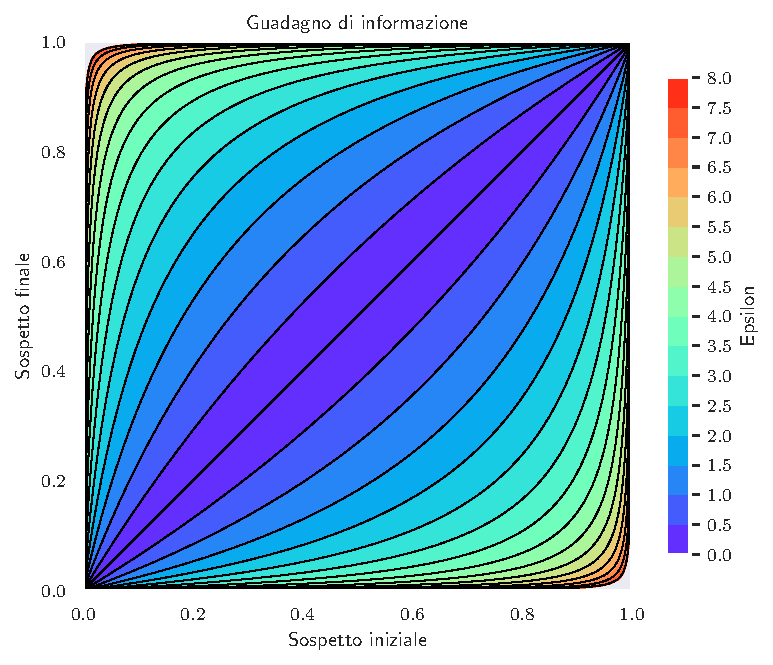
\includegraphics[scale=0.8]{plots/information_gain.pdf}
    \caption{Guadagno di informazione sul dataset al variare di epsilon}
\end{figure}

\section{Meccanismo di Laplace}
Le query più comuni che vengono effettuate su database sono di tipo numerico, precisamente sono funzioni del tipo $f \colon \mathbb{N}^{|\mathcal{X}|} \to \mathbb{R}^k$, dove $\mathcal{X}$ rappresenta l'universo di possibili record in un database $x$.

Per rendere questa tipologia di query differenzialmente privata con il meccanismo di Laplace si aggiunge rumore campionato da una distribuzione di Laplace:
\begin{align}
\label{eq:laplace_distribution}
    Lap(x|\mu,b) = \frac{1}{2b}\exp\left({-\frac{|x-\mu|}{b}}\right)
\end{align}

\begin{figure}[H]
    \centering
    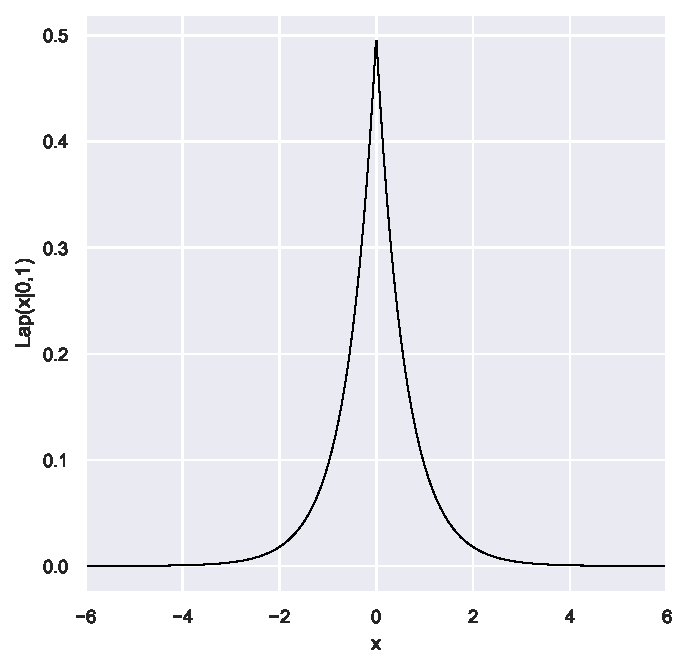
\includegraphics[scale=0.5]{plots/laplace_pdf.pdf}
    \caption{Distribuzione di Laplace}
\end{figure}

\subsection{Definizione}
Si consideri una qualsiasi funzione $f \colon \mathbb{N}^{|\mathcal{X}|} \to \mathbb{R}^k$, il meccanismo di Laplace è definito:
\begin{equation}
\label{eq:laplace_mechanism}
    \mathcal{M}_L(x, f(\cdot), \varepsilon) = f(x) + (Y_1, \dots, Y_k)
\end{equation}
dove i parametri $Y_i$ sono valori campionati da una distribuzione di Laplace. Per illustrare la calibrazione della distribuzione utilizzata è necessario introdurre alcuni concetti.

\subsubsection{Distanza tra database}
Si considerino due database $x, y \in \mathbb{R}^{|\mathcal{X}|}$.
Per definire la distanza tra i due database si fa uso della norma $\ell_1$, dove la norma $\ell_1$ di un database è definita come:
\begin{equation}
\label{eq:l1_norm}
    ||x||_1 = \sum_{i=1}^{|\mathcal{X}|} |x_i|
\end{equation}
La distanza $\ell_1$ tra due database $x$ e $y$ è $||x - y||_1$.

In questo caso $||x||_1$ è una misura del numero di record contenuti nel database e $||x - y||_1$ rappresenta quanti record sono diversi tra $x$ e $y$.

\subsubsection{Sensitività di una funzione}
La sensitività di una funzione è un valore che indica la magnitudine massima che un cambiamento dei dati di un singolo individuo può causare sul risultato della funzione considerata; questo valore verrà utilizzato come parametro per calibrare la quantità di rumore che il meccanismo aggiungerà ai risultati delle query.

La sensitività $\ell_1$ è definita come:
\begin{equation}
    \Delta f = \max_{\substack{x,y \in \mathbb{N}^{|\mathcal{X}|}\\||x - y||_1 = 1}} ||f(x) - f(y)||_1
\end{equation}

Utilizzando la sensitività della funzione in considerazione si calibra la scala (parametro $b$) della distribuzione di Laplace come $Lap(x|0,\Delta f/\varepsilon)$. Per la dimostrazione che l'utilizzo di questa distribuzione crea un meccanismo che rispetta $\varepsilon$-privacy differenziale consultare \ref{proof:laplace_mechanism}

\subsection{Limitazione del contributo}
Si supponga di avere a disposizione un dataset che raccoglie le lamentele poste dai clienti di un'azienda tramite un modulo di feedback e di voler creare un report sul numero di lamentele poste al giorno; si decide di applicare il meccanismo di Laplace per anonimizzare i risultati dell'analisi.

Il primo passo per creare un meccanismo di Laplace differenzialmente privato è calcolare la sensitività della funzione in considerazione. Dato che si tratta di un'operazione di conteggio, intuitivamente si può pensare che questo valore sia pari a 1; tuttavia è necessario considerare la \textit{contribuzione massima} che un singolo utente può apportare al conteggio per valutare correttamente casi in cui un individuo presenta più di una lamentela al giorno.

Se si considerasse $\Delta f = 1$ e quindi un parametro di scala per la distribuzione di Laplace pari a $b = \frac{1}{\varepsilon}$ si otterrebbe un meccanismo $x\varepsilon$-differenzialmente privato, dove $x$ corrisponde alla massima contribuzione che un singolo individuo può apportare al dataset. Supponendo un dataset di 500 unità con un utente che ha posto 5 lamentele, utilizzando $\Delta f = 1$ si otterrebbero due distribuzioni di probabilità con rapporto massimo di $e^{5\varepsilon}$, violando quindi la definizione di privacy differenziale.

Si riporta di seguito il grafico che mostra le due distribuzioni di probabilità e il loro rapporto.
\begin{figure}[H]
    \centering
    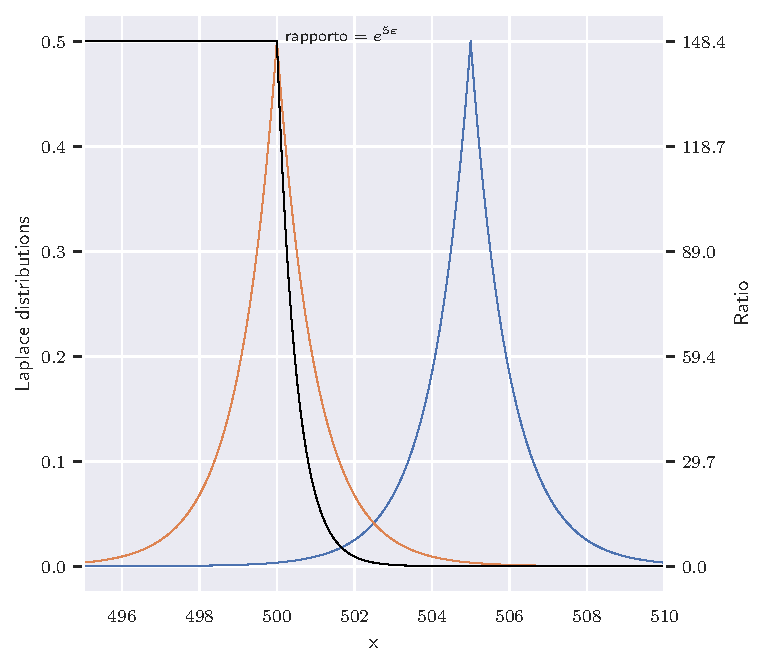
\includegraphics[scale=0.7]{plots/double_laplace_pdf.pdf}
    \caption{Distribuzioni di Laplace per dataset con e senza utente con multiple lamentele}
\end{figure}

Per rispettare i requisiti della privacy differenziale è necessario utilizzare la sensitività della funzione di conteggio che tiene conto della possibilità di avere multipli record legati a un singolo individuo.

\subsubsection{Scelta dei limiti}
Generalizzando, il problema ricade sulle caratteristiche del particolare dominio di applicazione, si rende quindi necessario l'intervento di un esperto del dominio allo scopo di definire un ragionevole limite massimo alla sensitività; in fase di analisi sarà necessario ignorare i record che portano il conteggio oltre il limite.







\newpage
Step successivi:\\
analisi fatta finora prevede un modello interattivo\\
considerazione su modello distribuito e locale\\
considerazione su caching e possibilità di ripetere query\\

\chapter{Meccanismi Differenzialmente Privati}

\section{Definizione}
La definizione seguente costituisce un formalismo più ristretto rispetto alla definizione completa, quest'ultima include un secondo parametro $\mathcal{\delta}$, la cui funzione e utilità verranno discusse in seguito.

Una trasformazione $\mathcal{M}$ è considerata $\varepsilon$-differenzialmente privata se, per ogni dataset $D_1$ e $D_2$ che differiscono al massimo per un individuo ($\norm{D_1 - D_2}_1 \le 1$) e ogni $S \subseteq \operatorname{Range}(\mathcal{M})$, vale la seguente disequazione \cite{10.1007/11681878_14}:
\begin{equation}
  \Pr[\mathcal{M}(D_1) = S] \le e^{\varepsilon} \cdot \Pr[\mathcal{M}(D_2) = S]
  \label{eq:e_differential_privacy}
\end{equation}

I termini $\Pr[\mathcal{M}(D_1) = S]$ e $\Pr[\mathcal{M}(D_2) = S]$ indicano la probabilità che il risultato dell'applicazione del meccanismo $\mathcal{M}$ su $D_1$ e $D_2$ risulti nell'output $S \in \operatorname{Range}(\mathcal{M})$.
Il termine $e^\varepsilon, \varepsilon > 0$ rappresenta un coefficiente che indica quanto le due probabilità possono differire tra di loro, in particolare per valori di $\varepsilon$ vicini a $0$ le probabilità sono simili; all'aumentare di $\varepsilon$ la differenza tra le due probabilità può aumentare.

Considerando che i due database $D_1$ e $D_2$ differiscono per un solo individuo, essi sono intercambiabili; ciò rende la definizione simmetrica. Vale quindi anche:
\begin{equation}
  e^{-\varepsilon} \cdot \Pr[\mathcal{M}(D_2) = S] \le \Pr[\mathcal{M}(D_1) = S] \le e^{\varepsilon} \cdot \Pr[\mathcal{M}(D_2) = S]
  \label{eq:e_differential_privacy_symm}
\end{equation}

\subsubsection{Un esempio pratico}
\label{ex:coint_toss}
Si supponga di volere condurre un sondaggio su una popolazione ponendo la domanda: "Nell'ultimo anno hai guidato un veicolo sotto l'influenza di alcol o stupefacenti?".
Ovviamente, una persona alla quale viene posta direttamente questa domanda tenderà a mentire allo scopo di proteggere la propria privacy e evitare di autoincriminarsi. In questa istanza può rendersi utile l'applicazione di un meccanismo differenzialmente privato.

Per ovviare a questa limitazione del processo di raccolta dati, si richiede ai partecipanti di lanciare una moneta senza mostrare il risultato:
\begin{itemize}
    \item se il risultato è testa il soggetto risponde alla domanda in modo sincero
    \item se il risultato è croce il soggetto lancia una seconda moneta: su testa risponde "Si", su croce "No"
\end{itemize}

\begin{tikzpicture}
\node (start) [draw,font=\scriptsize,rectangle,align=center,text width=0.2*\textwidth] {Nell'ultimo anno hai guidato un veicolo sotto l'influenza di alcol o stupefacenti?};

\node (dec1) [draw,font=\scriptsize,rectangle,right=2.5cm of start.center] {Lancia moneta};
\node (heads1) [draw,minimum height=1cm,minimum width=1cm,font=\scriptsize,circle,above=1cm of dec1.center] {Testa};
\node (tails1) [draw,minimum height=1cm,minimum width=1cm,font=\scriptsize,circle,below=1cm of dec1.center] {Croce};

\node (heads2) [draw,minimum height=1cm,minimum width=1cm,font=\scriptsize,circle,right=2cm of dec1.center] {Testa};
\node (truth) [draw,font=\scriptsize,rectangle,above=of heads2.north,right=2cm of heads1.center] {Verità};
\node (dec2) [draw,font=\scriptsize,rectangle,below=of heads2.south,right=2cm of tails1.east,anchor=center] {Lancia moneta};

\node (tails2) [draw,minimum height=1cm,minimum width=1cm,font=\scriptsize,circle,right=1cm of dec2.east] {Croce};
\node (out1) [draw,font=\scriptsize,rectangle,above=of tails2.north,right=of heads2.east] {Rispondi "Si"};
\node (out2) [draw,font=\scriptsize,rectangle,right=1cm of tails2.east] {Rispondi "No"};

\draw [-latex] (start.east) -- (dec1.west);
\draw [-latex] (dec1.north) -- (heads1.south);
\draw [-latex] (dec1.south) -- (tails1.north);
\draw [-latex] (tails1.east) -- (dec2.west);
\draw [-latex] (heads1.east) -- (truth.west);
\draw [-latex] (dec2.north) -- (heads2.south);
\draw [-latex] (dec2.east) -- (tails2.west);
\draw [-latex] (tails2.east) -- (out2.west);
\draw [-latex] (heads2.east) -- (out1.west);
\end{tikzpicture}

Questo processo introduce un elemento casuale alla risposta di un singolo soggetto, offrendo all'individuo una negazione plausibile contro eventuali accuse e impedendo a terze parti di discriminare sulla base delle risposte \cite{Warner01031965}.

Nel complesso, riscrivendo i risultati nei termini della definizione si ottiene:
\begin{itemize}
    \item $\Pr[\mathcal{M}(Si) = Si] = 0.75$, $\Pr[\mathcal{M}(Si) = No] = 0.25$
    \item $\Pr[\mathcal{M}(No) = Si] = 0.25$, $\Pr[\mathcal{M}(No) = No] = 0.75$
\end{itemize}

Considerati questi risultati si può affermare che il meccanismo illustrato è $\ln{3}$-differenzialmente privato; si può dimostrare partendo dalla definizione \eqref{eq:e_differential_privacy} che:
\begin{align*}
    \frac{\Pr[\mathcal{M}(D_1) = S]}{\Pr[\mathcal{M}(D_2) = S]
    } &\le e^{\varepsilon}\\
    \frac{\Pr[\mathcal{M}(Si) = Si]}{\Pr[\mathcal{M}(Si) = No]} &\le 3 = \frac{\Pr[\mathcal{M}(No) = No]}{\Pr[\mathcal{M}(No) = Si]}
\end{align*}

Il meccanismo illustrato dimostra in termini semplici come la privacy differenziale possa agire sui dati per proteggere la privacy dei partecipanti che aderiscono a essere inseriti in una raccolta di dati. Come specificato in precedenza, questo processo garantisce negazione plausibile sul contenuto della risposta ai soggetti partecipanti; non fornisce tuttavia la possibilità di negare di aver partecipato al sondaggio. Al contrario, la privacy differenziale è applicabile solamente a distribuzioni di dati basate su sistemi di interrogazione che generano risultati aggregati.

\subsection{Quantificazione della conoscenza dell'attaccante}
Il parametro $\varepsilon$ presente nella definizione di $\varepsilon$-DP può essere interpretato come una misura del livello massimo di conoscenza che un potenziale attaccante può guadagnare osservando i risultati di un'interrogazione del meccanismo differenzialmente privato.

Prendendo come riferimento un attaccante che conosce l'intero database eccetto il soggetto target si può modellare il suo punto di vista considerando due possibili dataset: $D_{in}$ contiene il target mentre $D_{out}$ no; l'obiettivo dell'attaccante è capire quale dei due database è quello reale.

Nel modello dell'attaccante si può esprimere il sospetto che il database $D$ sia $D_{in}$ come $\Pr[D = D_{in}] = 1 - \Pr[D = D_{out}]$. Si supponga ora che l'attaccante abbia osservato che il meccanismo DP applicato a $D$ restituisce l'output $O$: si può esprimere la probabilità che $D = D_{in}$ dopo aver osservato l'output come $\Pr[D = D_{in} | \mathcal{M}(D) = O]$; applicando il teorema di Bayes si ottiene un'espressione che permette di quantificare il livello di sospetto $Pr[D = D_{in}|M(D) = O]$ che l'attaccante ha dopo aver osservato l'output $O$.
\begin{equation}
\label{eq:bayes_susp}
    \Pr[D = D_{in} | \mathcal{M}(D) = O] = \frac{\Pr[D = D_{in}] \cdot \Pr[\mathcal{M}(D) = O | D = D_{in}]}{\Pr[\mathcal{M}(D) = O]}
\end{equation}
Il termine $\Pr[D = D_{in}]$ è il sospetto iniziale e il termine $\Pr[\mathcal{M}(D) = O | D = D_{in}]$ può essere riscritto come $\Pr[\mathcal{M}(D_{in}) = O]$ indicando la probabilità che il meccanismo $\mathcal{M}$ applicato a $D_{in}$ restituisca $O$. Mentre i primi due termini sono conosciuti, il termine $\Pr[\mathcal{M}(D) = O]$ è sconosciuto; per rimediare si può considerare il rapporto tra i due sospetti aggiornati all'output $O$.
\begin{equation}
\label{eq:bayes_susp_ratio}
    \frac{\Pr[D = D_{in} | \mathcal{M}(D) = O]}{\Pr[D = D_{out} | \mathcal{M}(D) = O]} = \frac{\Pr[D = D_{in}]}{\Pr[D = D_{out}]} \cdot \frac{\Pr[\mathcal{M}(D_{in}) = O]}{\Pr[\mathcal{M}(D_{out}) = O]}
\end{equation}
In questa espressione emerge il termine $\frac{\Pr[\mathcal{M}(D_{in}) = O]}{\Pr[\mathcal{M}(D_{out}) = O]}$, la definizione di $\varepsilon$-DP \eqref{eq:e_differential_privacy} limita il rapporto come segue:
\begin{equation}
\label{eq:e_dp_bounds}
    e^{-\varepsilon} \le \frac{\Pr[\mathcal{M}(D_{in}) = O]}{\Pr[\mathcal{M}(D_{out}) = O]} \le e^{\varepsilon}
\end{equation}
Applicando all'equazione \eqref{eq:bayes_susp_ratio} si ottiene:
\begin{equation}
\label{eq:mid_information_gain}
    e^{-\varepsilon} \cdot \frac{\Pr[D = D_{in}]}{\Pr[D = D_{out}]} \le \frac{\Pr[D = D_{in} | \mathcal{M}(D) = O]}{\Pr[D = D_{out} | \mathcal{M}(D) = O]} \le e^{\varepsilon} \cdot \frac{\Pr[D = D_{in}]}{\Pr[D = D_{out}]} 
\end{equation}
Applicando le sostituzioni $\Pr[D = D_{out}] = 1 - \Pr[D = D_{in}]$ e $\Pr[D = D_{out} | \mathcal{M}(D) = O] = 1 - \Pr[D = D_{in} | \mathcal{M}(D) = O]$ e riorganizzando i termini si ottiene:
\begin{equation}
\label{eq:information_gain}
    \frac{\Pr[D = D_{in}]}{e^\varepsilon + (1 - e^\varepsilon) \cdot \Pr[D = D_{in}]} \le \Pr[D = D_{in} | \mathcal{M}(D) = O] \le \frac{e^\varepsilon \cdot \Pr[D = D_{in}]}{1 + (e^\varepsilon - 1) \cdot \Pr[D = D_{in}]}
\end{equation}
Per i passaggi della trasformazione, consultare l'appendice \ref{eqd:information_gain_derivation}.

Tracciando il grafico dell'espressione risultante al variare di $\varepsilon$ si può notare come il guadagno di informazione potenziale possa aumentare drasticamente per valori di $\varepsilon$ alti.
\begin{figure}[H]
    \centering
    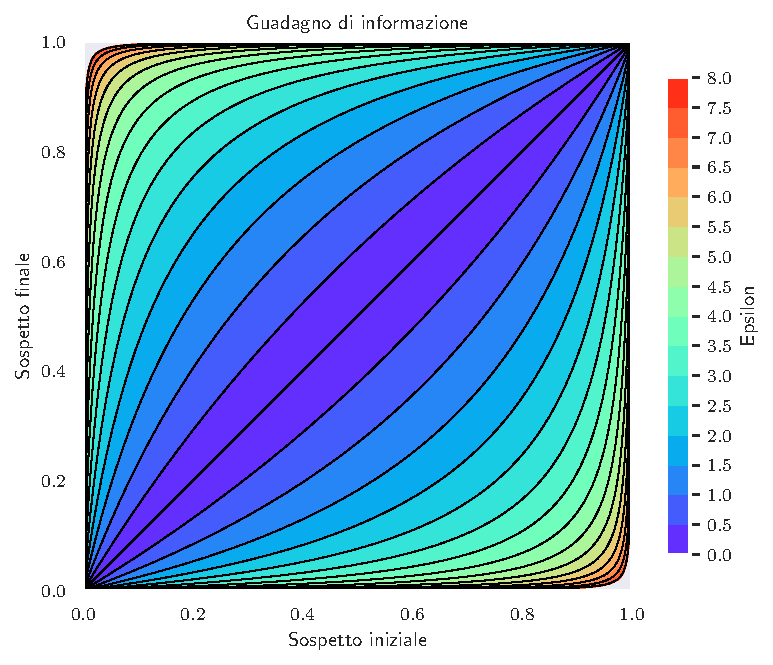
\includegraphics[scale=0.8]{plots/information_gain.pdf}
    \caption{Guadagno di informazione sul dataset al variare di epsilon}
\end{figure}

\section{Meccanismo di Laplace}
Le query più comuni che vengono effettuate su database sono di tipo numerico, precisamente sono funzioni del tipo $f \colon \mathbb{N}^{|\mathcal{X}|} \to \mathbb{R}^k$, dove $\mathcal{X}$ rappresenta l'universo di possibili record in un database $x$.

Per rendere questa tipologia di query differenzialmente privata con il meccanismo di Laplace si aggiunge rumore campionato da una distribuzione di Laplace:
\begin{align}
\label{eq:laplace_distribution}
    Lap(x|\mu,b) = \frac{1}{2b}\exp\left({-\frac{|x-\mu|}{b}}\right)
\end{align}

\begin{figure}[H]
    \centering
    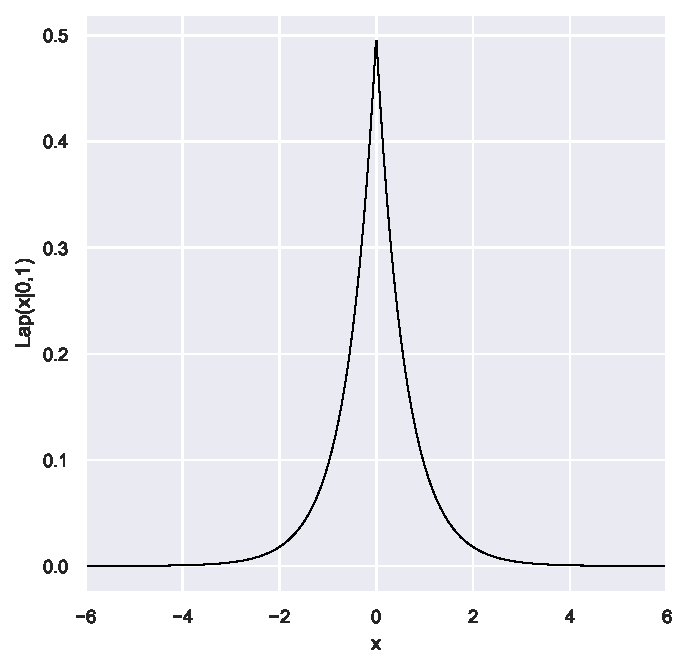
\includegraphics[scale=0.5]{plots/laplace_pdf.pdf}
    \caption{Distribuzione di Laplace}
\end{figure}

\subsection{Definizione}
Si consideri una qualsiasi funzione $f \colon \mathbb{N}^{|\mathcal{X}|} \to \mathbb{R}^k$, il meccanismo di Laplace è definito:
\begin{equation}
\label{eq:laplace_mechanism}
    \mathcal{M}_L(x, f(\cdot), \varepsilon) = f(x) + (Y_1, \dots, Y_k)
\end{equation}
dove i parametri $Y_i$ sono valori campionati da una distribuzione di Laplace. Per illustrare la calibrazione della distribuzione utilizzata è necessario introdurre alcuni concetti.

\subsubsection{Distanza tra database}
Si considerino due database $x, y \in \mathbb{R}^{|\mathcal{X}|}$.
Per definire la distanza tra i due database si fa uso della norma $\ell_1$, dove la norma $\ell_1$ di un database è definita come:
\begin{equation}
\label{eq:l1_norm}
    ||x||_1 = \sum_{i=1}^{|\mathcal{X}|} |x_i|
\end{equation}
La distanza $\ell_1$ tra due database $x$ e $y$ è $||x - y||_1$.

In questo caso $||x||_1$ è una misura del numero di record contenuti nel database e $||x - y||_1$ rappresenta quanti record sono diversi tra $x$ e $y$.

\subsubsection{Sensitività di una funzione}
La sensitività di una funzione è un valore che indica la magnitudine massima che un cambiamento dei dati di un singolo individuo può causare sul risultato della funzione considerata; questo valore verrà utilizzato come parametro per calibrare la quantità di rumore che il meccanismo aggiungerà ai risultati delle query.

La sensitività $\ell_1$ è definita come:
\begin{equation}
    \label{eq:sensitivity}
    \Delta f = \max_{\substack{x,y \in \mathbb{N}^{|\mathcal{X}|}\\||x - y||_1 = 1}} ||f(x) - f(y)||_1
\end{equation}

Utilizzando la sensitività della funzione in considerazione si calibra la scala (parametro $b$) della distribuzione di Laplace come $Lap(x|0,\Delta f/\varepsilon)$. Per la dimostrazione che l'utilizzo di questa distribuzione crea un meccanismo che rispetta $\varepsilon$-privacy differenziale consultare \ref{proof:laplace_mechanism}

\subsection{Meccanismo di Laplace e singole statistiche}
Si supponga di avere a disposizione un dataset che raccoglie le lamentele poste dai clienti di un'azienda tramite un modulo di feedback e di voler creare un report sul numero di lamentele poste al giorno; si decide di applicare il meccanismo di Laplace che aggiunge rumore calibrato per anonimizzare i risultati dell'analisi.

Il primo passo per creare un meccanismo di Laplace differenzialmente privato è calcolare la sensitività della funzione in considerazione. Dato che si tratta di un'operazione di conteggio, intuitivamente si può pensare che questo valore sia pari a 1; tuttavia è necessario considerare la \textit{contribuzione massima} che un singolo utente può apportare al conteggio per valutare correttamente casi in cui un individuo presenta più di una lamentela al giorno.

Se si considerasse $\Delta f = 1$ e quindi un parametro di scala per la distribuzione di Laplace pari a $b = \frac{1}{\varepsilon}$ si otterrebbe un meccanismo $x\varepsilon$-differenzialmente privato, dove $x$ corrisponde alla massima contribuzione che un singolo individuo può apportare al dataset. Supponendo un dataset di 500 unità con un utente che ha posto 5 lamentele, utilizzando $\Delta f = 1$ si otterrebbero due distribuzioni di probabilità con rapporto massimo di $e^{5\varepsilon}$, violando quindi la definizione di privacy differenziale.

Si riporta di seguito il grafico che mostra le due distribuzioni di probabilità centrate sul numero di soggetti nei due database, uno con il soggetto con le 5 lamentele e l'altro senza, e il loro rapporto.
\begin{figure}[H]
    \centering
    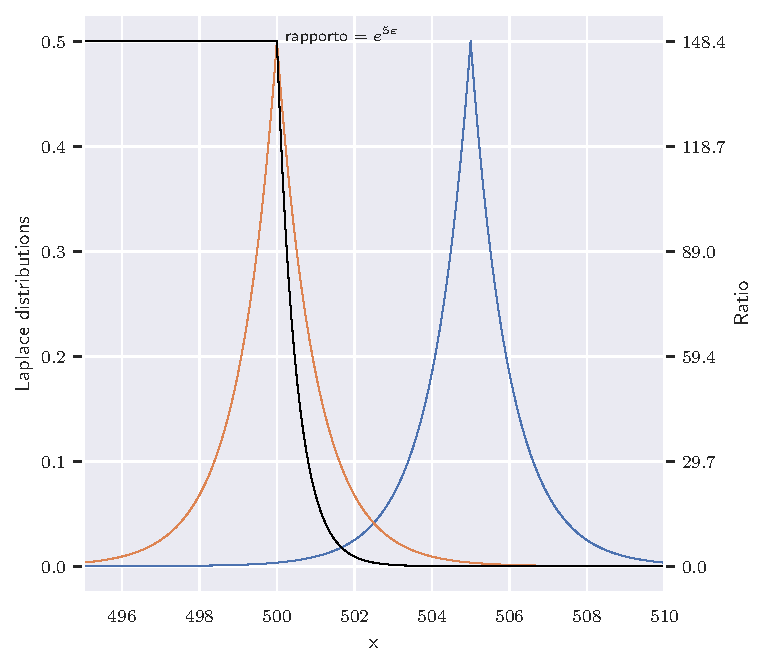
\includegraphics[scale=0.7]{plots/double_laplace_pdf.pdf}
    \caption{Distribuzioni di Laplace per dataset con e senza utente con multiple lamentele}
\end{figure}

Per rispettare i requisiti della privacy differenziale è necessario utilizzare la sensitività della funzione di conteggio tenendo conto della possibilità di avere multipli record legati a un singolo individuo.

\subsubsection{Limitazione del contributo}
\label{sec:contribution_lim}
Generalizzando, il problema ricade sulle caratteristiche del particolare dominio di applicazione; si rende quindi necessario l'intervento di un esperto del dominio allo scopo di definire un ragionevole limite massimo alla sensitività; in fase di analisi sarà necessario limitare il conteggio dei record relativi a un singolo individuo.

\subsection{Meccanismo di Laplace e statistiche multiple}
Nel caso in cui si vogliano rilasciare statistiche multiple su un dataset (e.g. istogrammi) è necessario considerare come viene applicato il rumore a ognuna delle statistiche o categorie calcolate per assicurarsi di non violare la definizione di privacy differenziale.

Si distinguono due casistiche differenti: un caso è caratterizzato da utenti che possono influenzare al massimo una statistica, che è quindi in questo senso disgiunta dalle altre, e un caso dove gli utenti possono influenzare diverse statistiche.

\subsubsection{Caso 1: statistiche disgiunte}
Quando le statistiche multiple da includere nella distribuzione di dati sono disgiunte, è sufficiente aggiungere rumore estratto da una distribuzione di Laplace di scala $\frac{\Delta f}{\varepsilon}$ a ogni statistica calcolata. Un esempio di questa eventualità è la creazione di un istogramma che mostra la distribuzione di età in un dataset.

\begin{figure}[H]
    \begin{subfigure}[t]{.5\textwidth}
        \centering
        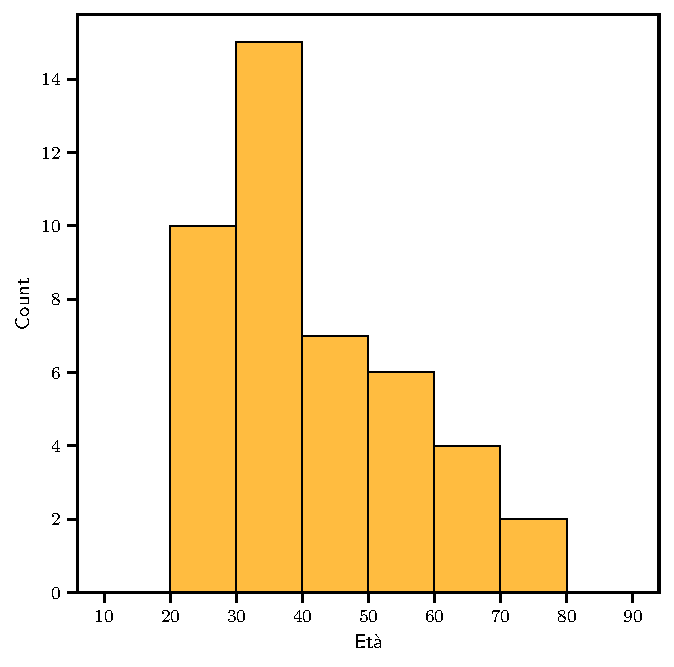
\includegraphics[width=.8\linewidth]{plots/age_histogram.pdf}
        \caption{Distribuzione età soggetti}
    \end{subfigure}
    \begin{subfigure}[t]{.5\textwidth}
        \centering
        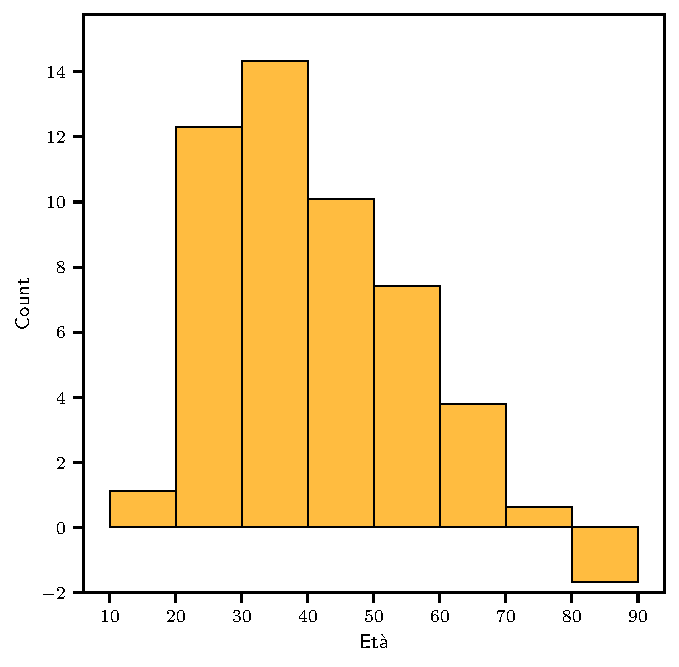
\includegraphics[width=.8\linewidth]{plots/age_histogram_negative.pdf}
        \caption{Distribuzione differenzialmente privata}
    \end{subfigure}
\end{figure}

Il grafico di sinistra rappresenta i dati senza nessuna strategia di anonimizzazione, si crea il secondo istogramma utilizzando un meccanismo di Laplace con scala $\frac{1}{\varepsilon}$ che aggiunge rumore a ogni categoria utilizzando lo stesso parametro di scala. Come si può notare dai due grafici, ci sono evidenti problemi con la categoria 80-89 in quanto risulta negativa, così come con le altre categorie perché presentano valori non interi; in questo caso l'applicazione del meccanismo di Laplace ha dato luogo a valori incongruenti.

Per fare fronte a casi come questo in cui l'applicazione del meccanismo differenzialmente privato scelto porta i dati al di fuori del loro dominio (e.g. valori negativi per un conteggio, valori non interi) è lecito applicare funzioni di post-processing. 

Considerando un meccanismo $\varepsilon$-differenzialmente privato $\mathcal{M} \colon \mathbb{N}^{|\mathcal{X}|} \to \mathbb{R}$ e un mapping casuale arbitrario $f \colon \mathbb{R} \to \mathbb{R}'$ allora $f \circ \mathcal{M} \colon \mathbb{N}^{|\mathcal{X}|} \to \mathbb{R}'$ è anch'esso $\varepsilon$-differenzialmente privato. Questo risultato è dimostrato formalmente in \cite{TCS-042}, tuttavia intuitivamente si può capire che una qualsiasi funzione di post-processing che applica una trasformazione ai dati non agisce sui dati del dataset originario, non può quindi aumentare la perdita di privacy che la privacy differenziale concede con il meccanismo utilizzato.

Applicando all'esempio di prima gli opportuni arrotondamenti e rimpiazzando i valori negativi con 0 si ottiene nuovamente una distribuzione di dati $\varepsilon$-differenzialmente privata.

\begin{figure}[H]
    \centering
    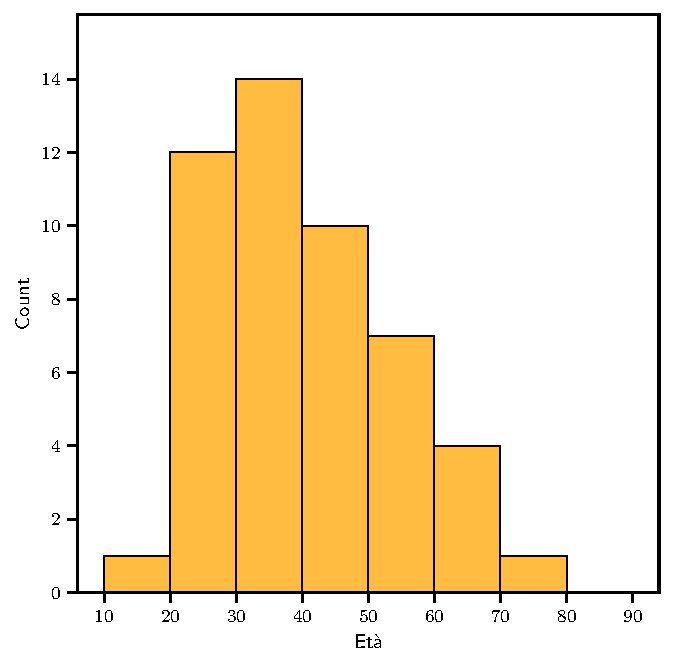
\includegraphics[width=.4\linewidth]{plots/age_histogram_negative_post_processed.pdf}
    \caption{Distribuzione differenzialmente privata con post-processing applicato}
\end{figure}

\subsubsection{Caso 2: statistiche intersecanti}
Se le diverse statistiche da rilasciare possono essere influenzate dallo stesso utente, dato un numero $C$ di statistiche sarà necessario calcolare la sensitività della funzione considerando quanto un singolo utente possa contribuire a tutte le statistiche, nel caso di conteggi o calcolo di medie sarà necessario considerare $\Delta f = C$ e un parametro di scala $b = C / \varepsilon$, in questo modo ogni statistica sarà $\varepsilon / C$-differenzialmente privata.

Questa strategia porta a evidenziare il vero significato del parametro $\varepsilon$ come un valore che quantifica il \textbf{budget di privacy} assegnato a una particolare distribuzione di dati.

Una soluzione più flessibile rispetto a quella di creare $C$ statistiche $\varepsilon / C$-DP è quella di suddividere il budget in parti diseguali $\varepsilon_1, \varepsilon_2, \dots, \varepsilon_C$ tale che $\sum_{i=1}^{C} \varepsilon_i = \varepsilon$. Se esistono statistiche che sono più sensibili al rumore o necessitano di essere più accurate, è possibile allocare una porzione di budget maggiore: questo risulterà nell'aggiunta di una quantità di rumore minore, tuttavia sarà necessario aggiungere più rumore alle altre statistiche.

\section{\texorpdfstring{$(\varepsilon,\delta)$}{TEXT}-privacy differenziale}
Si supponga di procedere con un sondaggio che pone domande ai soggetti senza un numero predefinito di possibili risposte e che può quindi dare vita a un numero di categorie non prestabilito.

Questo tipo di raccolta di dati è intrinsecamente soggetto a distorsioni, imprecisioni e, in generale, rumore nei dati raccolti, come ad esempio risposte di soggetti che fraintendono la domanda, risposte intenzionalmente non valide o semplicemente risposte rare.

Il problema che sorge in questi casi consiste nella possibilità di avere due database che differiscono per un solo soggetto, ma uno dei due perde una categoria rara.

\begin{figure}[H]
    \begin{subfigure}[t]{.5\textwidth}
        \centering
        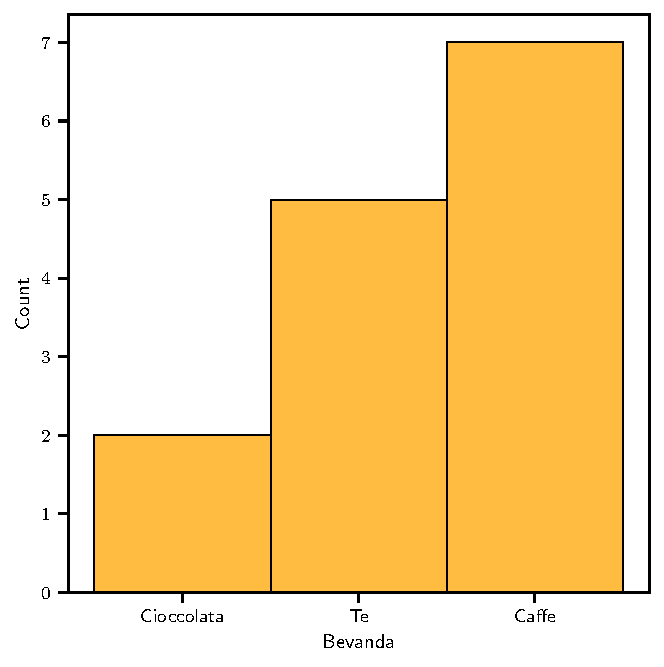
\includegraphics[width=.8\linewidth]{plots/drink_histogram_no_matcha.pdf}
        \caption{Distribuzione bevande database 1}
    \end{subfigure}
    \begin{subfigure}[t]{.5\textwidth}
        \centering
        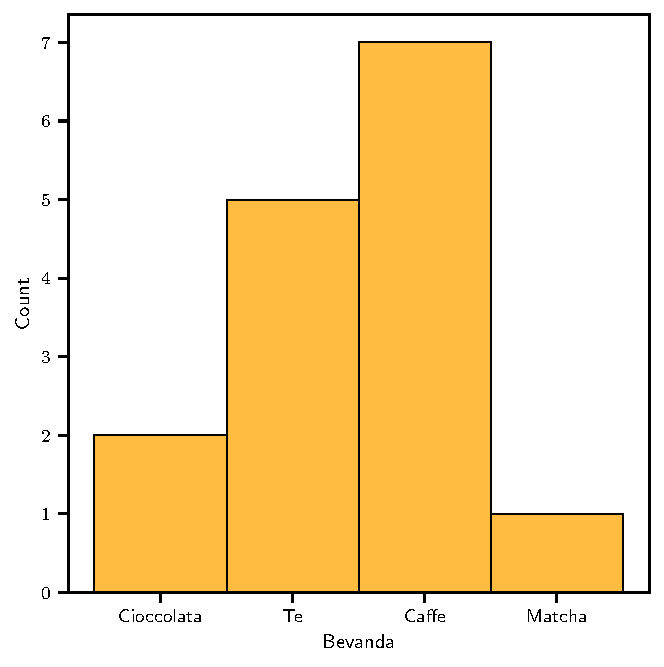
\includegraphics[width=.8\linewidth]{plots/drink_histogram_yes_matcha.pdf}
        \caption{Distribuzione bevande database 2}
    \end{subfigure}
\end{figure}

Un attaccante che osserva questi risultati è in grado di capire con totale certezza quale dei due database contiene il soggetto di interesse: questo è un \textbf{evento distintivo}.

Una possibile soluzione consiste nell'applicare una soglia minima: si aggiunge rumore a tutte le categorie che sono state generate dalla raccolta di dati per poi scartare quelle che ricadono sotto a questa soglia per evitare \textit{eventi distintivi} che possono infrangere la definizione di DP.

Nell'esempio di prima si potrebbe scegliere una soglia conservativa pari a 2, ottenendo come risultato il seguente istogramma.

\begin{figure}[H]
    \centering
    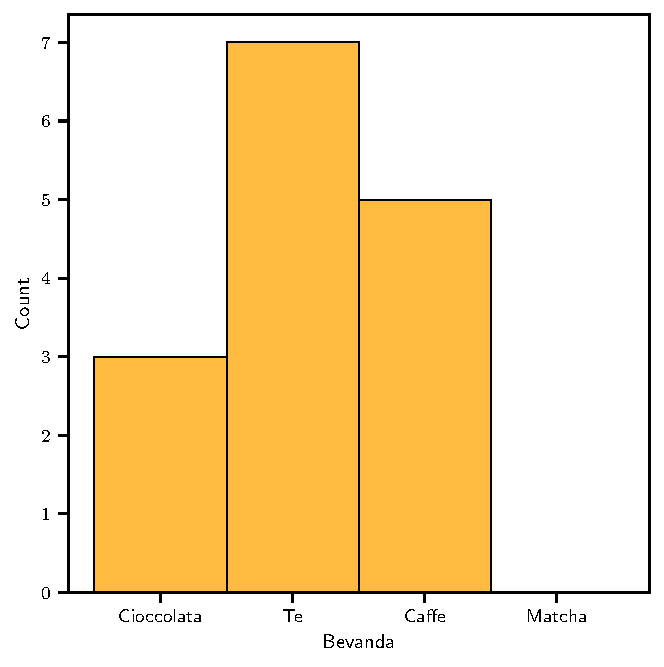
\includegraphics[width=.4\linewidth]{plots/drink_histogram_yes_matcha_threshold.pdf}
    \caption{Distribuzione differenzialmente privata con soglia applicata (>= 2)}
\end{figure}

Questa soluzione non è perfetta, come si può vedere, la categoria rara "Matcha" viene rimossa dalla distribuzione di dati finale; la categoria "Cioccolata" tuttavia, pur ricadendo sotto la soglia nel dataset originario, è stata pubblicata in quanto l'aggiunta di rumore dal meccanismo DP risulta sopra la soglia, questo caso viola la definizione di $\varepsilon$-DP.

\subsection{Definizione}
Per poter modellare una versione di DP che sia in grado di comprendere release di dati più vicine a casi realistici è necessario introdurre una nuova definizione: $(\varepsilon, \delta)$-privacy differenziale, definizione che rilassa lo standard imposto dalla definizione di $(\varepsilon)$-DP introducendo il parametro $\boldsymbol{\delta}$. Questo termine può essere interpretato come la probabilità di pubblicare un evento distintivo.

\begin{equation}
    \Pr[\mathcal{M}(D_1) \in S] \le e^{\varepsilon} \cdot \Pr[\mathcal{M}(D_2) \in S] + \boldsymbol{\delta}
    \label{eq:ed_differential_privacy}
\end{equation}

Nell'esempio di prima si fa utilizzo di un meccanismo $(\varepsilon, \delta)$-DP con rumore campionato da una distribuzione di Laplace con una soglia pari a 2. Per stabilire quale parametro $\delta$ è stato utilizzato si calcola la probabilità che una categoria con conteggio 1, quindi esistente, superi la soglia utilizzata all'aggiunta di rumore di Laplace.

A questo scopo si fa uso della \textit{funzione di sopravvivenza} della variabile aleatoria da cui si campiona il rumore per il meccanismo; data una variabile aleatoria $X$ con funzione cumulativa di distribuzione $F(x)$, la funzione di sopravvivenza è definita come $S(x) = 1 - F(x) =  P[X > x]$.

\begin{figure}[H]
    \centering
    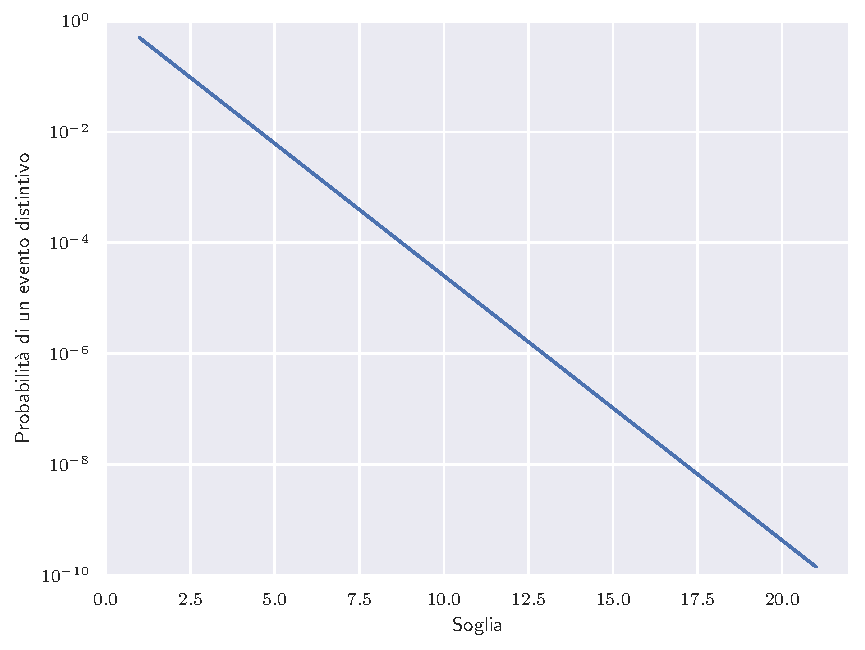
\includegraphics[width=.6\linewidth]{plots/threshold_probability.pdf}
    \caption{Parametro $\delta$ al variare della soglia}
\end{figure}

Dato che il parametro $\delta$ rappresenta la probabilità che un singolo utente ha di avere i propri dati esposti a seguito di una query al meccanismo DP, per questo viene spesso scelto $\delta \ll 1/n$ in quanto la probabilità che i dati di \textit{almeno un soggetto} vengano esposti è pari a $n\delta$: è necessario assicurarsi che questo valore sia abbastanza piccolo. Questa regola assume che i singoli eventi distintivi siano non correlati, spesso questo non è vero in realtà, ma è un'ottima approssimazione in pratica.
Ad esempio, in un database con 1 milione di utenti basterebbe una soglia di 15 per ottenere un valore di $n\delta < 0.1$.

\subsection{Perdita di privacy}

Riprendendo la definizione di guadagno di informazione \ref{eq:bayes_susp_ratio} con un meccanismo $\mathcal{M}$ definito $\varepsilon$-DP si può definire la seguente quantità.

\begin{equation}
     \frac{\Pr[\mathcal{M}(D_{in}) = O]}{\Pr[\mathcal{M}(D_{out}) = O]} = \frac{\frac{\Pr[D = D_{in} | \mathcal{M}(D) = O]}{\Pr[D = D_{out} | \mathcal{M}(D) = O]}}{\frac{\Pr[D = D_{in}]}{\Pr[D = D_{out}]}}
\end{equation}

Combinando questa definizione bayesiana del guadagno di informazione dopo l'osservazione dell'output $O$ con la definizione \ref{eq:e_differential_privacy} che impone $\frac{\Pr[\mathcal{M}(D_{in}) = O]}{\Pr[\mathcal{M}(D_{out}) = O]} \le e^\varepsilon$ si ottiene:

\begin{equation}
    \mathcal{L}_{D_{in},D_{out}}(O) = \ln \left(\frac{\Pr[\mathcal{M}(D_{in}) = O]}{\Pr[\mathcal{M}(D_{out}) = O]}\right)
\end{equation}

Questa quantità è definita come \textit{variabile aleatoria della perdita di privacy} (PLRV) al variare di $O$ e rappresenta il vero valore effettivo che $\varepsilon$ assume per un dato output $O$.

Prendendo un parametro $\varepsilon = \ln (3)$ e utilizzando una distribuzione di Laplace, si traccia il grafico di $e^{\mathcal{L}}$ ponendo sulle ascisse gli eventi a seconda della loro probabilità, evidenziando come la perdita di privacy non superi mai $e^\varepsilon$.

Si includono nel grafico anche 3 possibili output arbitrari considerando un dataset di 1000 individui.

\begin{figure}[H]
    \begin{subfigure}[t]{.5\textwidth}
        \centering
        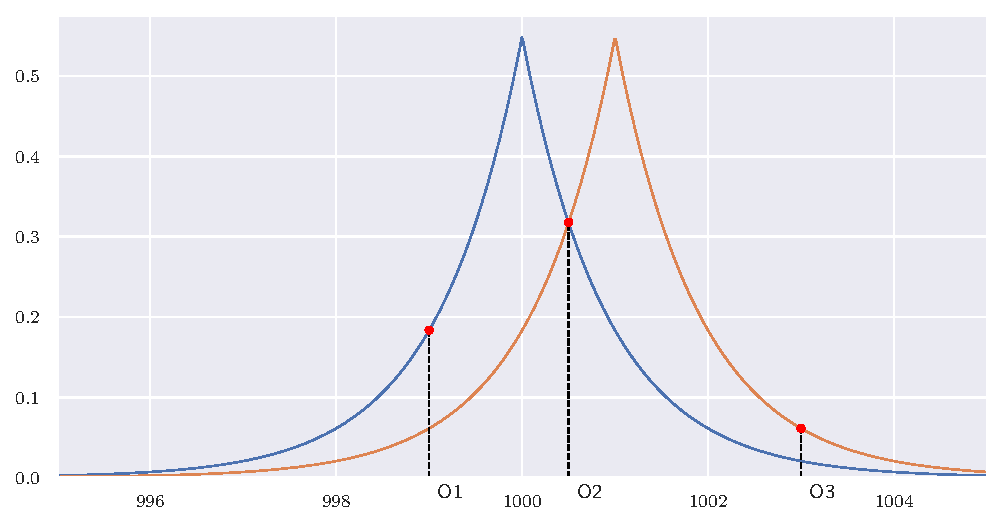
\includegraphics[width=\linewidth]{plots/laplace_plrv_two_dists.pdf}
        \caption{Distribuzioni di Laplace per database $D_{in}$ e $D_{out}$}
        \label{plot:plrv_two_dists}
    \end{subfigure}
    \begin{subfigure}[t]{.5\textwidth}
        \centering
        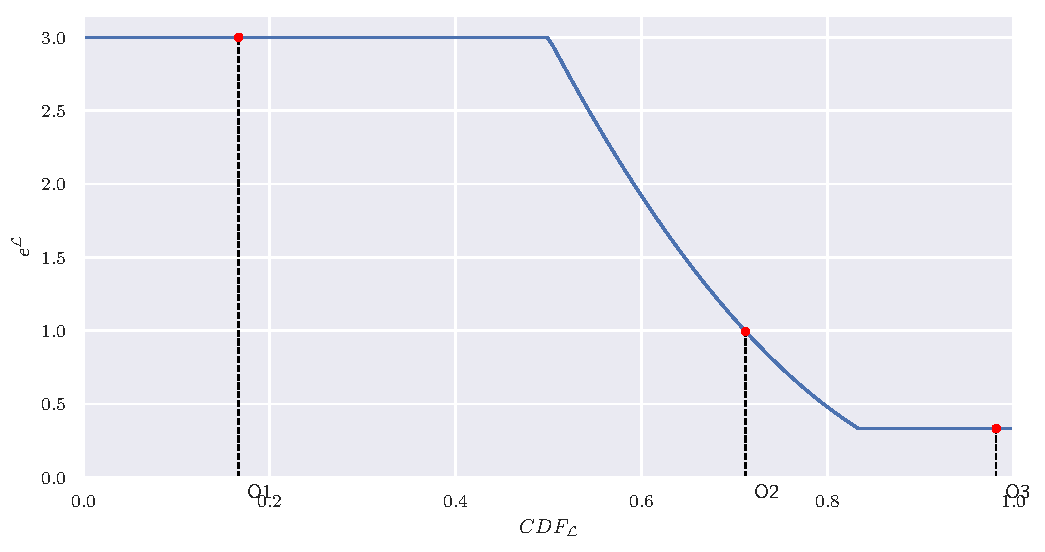
\includegraphics[width=\linewidth]{plots/laplace_e^plrv.pdf}
        \caption{Quantità di perdita di privacy al variare della probabilità degli eventi}
        \label{plot:e^prlv}
    \end{subfigure}
    \label{plot:plrv}
\end{figure}

Il grafico mostra chiaramente come la conoscenza di un possibile attaccante cambia a seconda di quale output viene osservato:
\begin{itemize}
    \item $\boldsymbol{O_1}$: è più probabile che questo output possa provenire da $D_{in}$ che $D_{out}$, di preciso esattamente 3 volte più probabile come mostrato nel grafico \ref{plot:e^prlv}.
    \item $\boldsymbol{O_2}$: è equamente probabile che l'output possa provenire da $D_{in}$ o da $D_{out}$.
    \item $\boldsymbol{O_3}$: è più probabile che l'output possa provenire dal database $D_{out}$, in questo caso la conoscenza dell'attaccante è divisa per 3 in quanto il vero database è $D_{in}$. 
\end{itemize}

Allo scopo di evidenziare e visualizzare il preciso significato del parametro $\delta$ nella definizione di $(\varepsilon, \delta)$-DP, si introduce un nuovo meccanismo DP che fa uso di rumore campionato da una \textit{distribuzione di Gauss}; in seguito si motiverà l'esistenza di tale meccanismo DP nel contesto del rilascio di multiple statistiche.

Riprendendo l'esempio precedente ma utilizzando distribuzioni gaussiane come base del meccanismo si ottengono i due grafici seguenti:

\begin{figure}[H]
    \begin{subfigure}[t]{.5\textwidth}
        \centering
        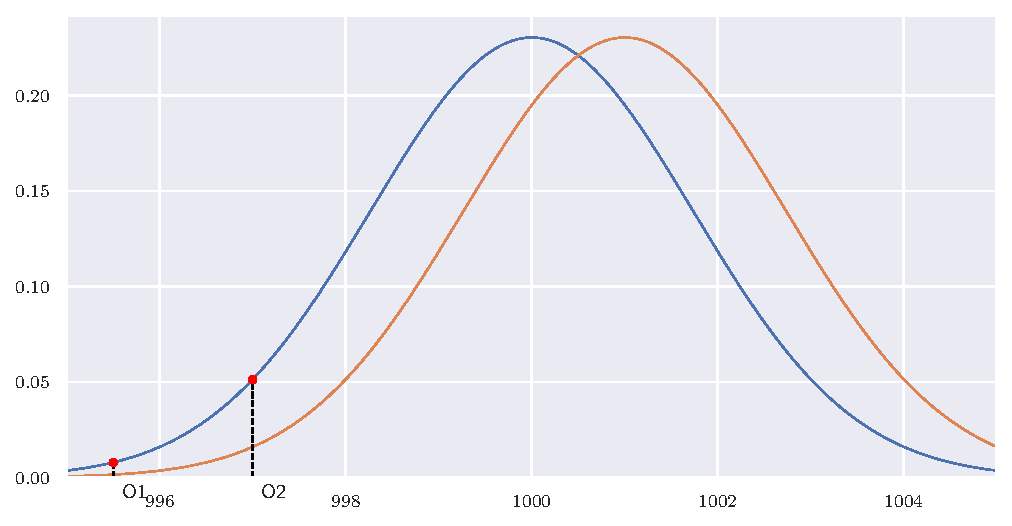
\includegraphics[width=\linewidth]{plots/normal_plrv_two_dists.pdf}
        \caption{Distribuzioni gaussiane per database $D_{in}$ e $D_{out}$}
        \label{plot:norm_plrv_two_dists}
    \end{subfigure}
    \begin{subfigure}[t]{.5\textwidth}
        \centering
        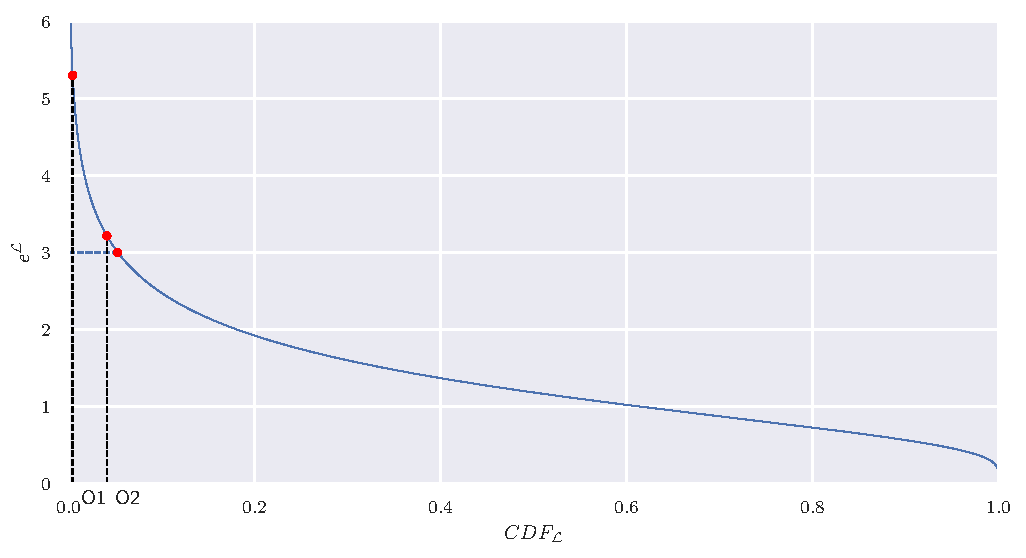
\includegraphics[width=\linewidth]{plots/normal_e^plrv.pdf}
        \caption{Quantità di perdita di privacy al variare della probabilità degli eventi}
        \label{plot:norm_e^prlv}
    \end{subfigure}
    \label{plot:plrv}
\end{figure}

Come si può vedere dal grafico di destra, con rumore gaussiano non esiste un limite superiore alla possibile perdita di privacy; la probabilità che si verifichi un evento distintivo è la probabilità che l'output restituito abbia un valore $e^{\mathcal{L}(O)} > 3$ e in questo caso è $\delta_1 \approx 0.053$, quindi il meccanismo è $(\ln (3), \delta_1)$-DP.

Pur essendo una caratterizzazione precisa del parametro $\delta$, questo metodo non dà il giusto peso agli eventi molto più significativi degli altri; alcuni eventi, quelli \textit{vicini} a $\delta_1$, hanno un effetto molto minore sulla perdita di privacy con un aumento esponenziale man mano che l'evento si avvicina a una probabilità cumulativa pari a 0.

Per tenere conto di questa caratteristica degli eventi quasi distintivi si rielabora la curva della PLRV prendendone l'inverso per posizionare gli eventi con maggiore perdita di privacy vicino a $y = 0$, si normalizza poi la curva prendendo il rapporto $\frac{e^\varepsilon}{e^\mathcal{L}}$ per portare gli eventi non estremi vicino a $y = 1$.

\begin{figure}[H]
    \centering
    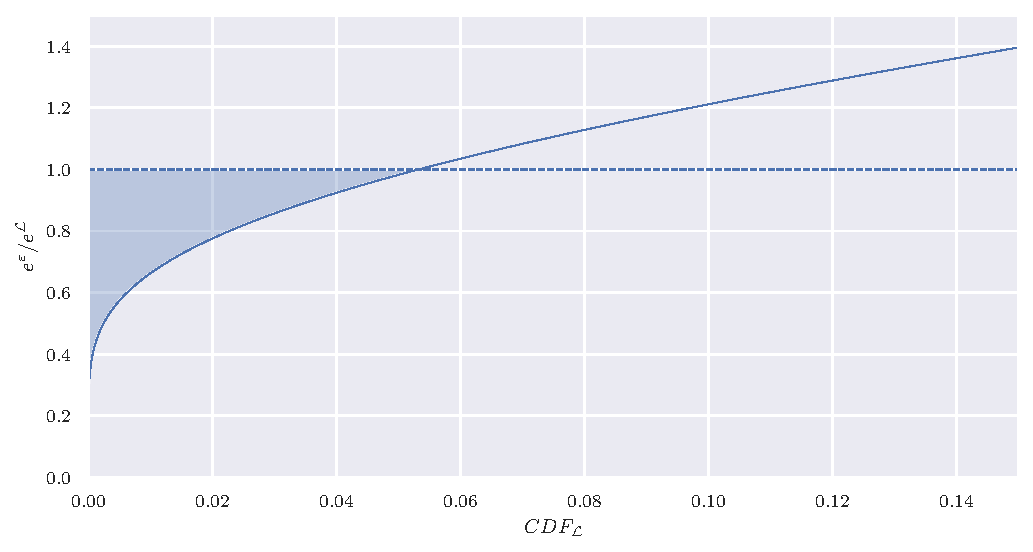
\includegraphics[width=.7\linewidth]{plots/normal_inverse_normalized_plrv.pdf}
    \caption{Inversa normalizzata della PLRV}
    \label{plot:normalized_inv_plrv}
\end{figure}

Questa trasformazione della curva della PLRV identifica l'effettivo valore di $\delta$ come l'area sottesa tra la retta $y = 1$, ovvero il limite che separa eventi quasi distintivi da rilasci di dati che rispettano $\varepsilon$-DP, e la curva $e^{\mathcal{\varepsilon}}/e^{\mathcal{L}}$ evidenziata nel grafico.

Per una dimostrazione che questa caratterizzazione identifica il valore di $\delta$ pesato sulla probabilità che $A(D_{in}) = O$ per ogni output $O$ consultare l'appendice \ref{proof:plrv_gaussian}.

\subsection{Rumore gaussiano}

Nella sezione precedente è stato utilizzato un meccanismo DP fondato sulla distribuzione normale per spiegare il significato del parametro $\delta$ nella definizione di $(\varepsilon, \delta)$-DP, di seguito si discuterà per quale motivo è desiderabile creare meccanismi di questo tipo anche se ricadono in una categoria di meccanismi DP con garanzie minori rispetto a quelle della $\varepsilon$-privacy differenziale.

La distribuzione gaussiana ha proprietà convenienti, ad esempio può essere usata per modellare variabili aleatorie con distribuzione sconosciuta in quanto una somma di molte variabili aleatorie porta a una distribuzione normale (teorema del limite centrale); un altro vantaggio è la regola delle tre sigma \cite{Kazmier_2003} che afferma che una variabile aleatoria campionata da questa distribuzione sarà:
\begin{itemize}
    \item nell'intervallo $[-\sigma, \sigma]$ 68\% delle volte;
    \item nell'intervallo $[-2\sigma, 2\sigma]$ 95\% delle volte;
    \item nell'intervallo $[-3\sigma, 3\sigma]$ 99.7\% delle volte.
\end{itemize}

Confrontando questa distribuzione con la distribuzione di Laplace si nota che le code della funzione di distribuzione diminuiscono molto più velocemente nella prima; prendendo $1000000$ di campioni dalle due distribuzioni, questi ricadranno nell'intervallo $[-5\sigma, 5\sigma]$ neanche 1\% delle volte nella distribuzione di Laplace e il 99.99...\% (12 volte 9) delle volte in una distribuzione normale.


\begin{figure}[H]
    \centering
    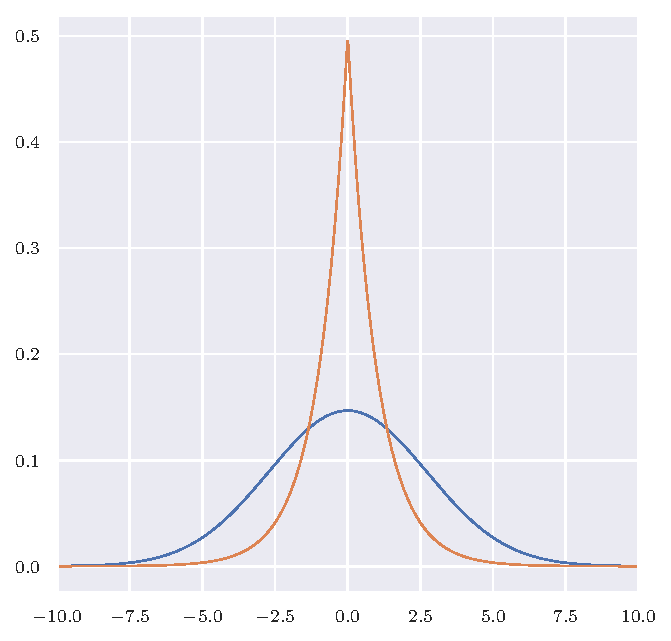
\includegraphics[width=.5\linewidth]{plots/gauss_laplace_e_1.pdf}
    \caption{Distribuzioni di Laplace e normale a confronto, $\varepsilon = 1, \delta = 10^{-5}$}
    \label{plot:normalized_inv_plrv}
\end{figure}

Mentre la distribuzione di Laplace è ideale quando si vogliono rilasciare poche statistiche poiché garantisce $\varepsilon$-DP, la distribuzione normale risulta utile quando si vogliono rilasciare numeri elevati di statistiche in quanto, come si può vedere dal grafico, utilizzando una distribuzione normale è necessario aggiungere più rumore rispetto a una distribuzione di Laplace.





\newpage
Step successivi:\\
analisi fatta finora prevede un modello interattivo\\
considerazione su modello distribuito e locale\\
considerazione su caching e possibilità di ripetere query\\
\chapter{GoDP - Strumento CLI per la creazione di release DP}
In questo capitolo si discuterà la creazione di un'applicazione per la generazione di distribuzioni di dati differenzialmente privati.

L'applicazione sfrutta la libreria Privacy on Beam sviluppata da Google \cite{pbeampac91:online} e basata sul framework Apache Beam; la scelta di questa libreria è motivata dal fatto che Privacy on Beam è tra le implementazioni open source di algoritmi DP più diffuse e perché mette a disposizione una vasta gamma di primitive DP.

Si è scelto di utilizzare un framework DP basato su Apache Beam per l'implementazione di \texttt{GoDP} per il repertorio di caratteristiche che garantiscono flessibilità per compiti di elaborazione dati.

Tra queste caratteristiche figura l'unificazione del modello di programmazione tra batch processing e stream processing con apposite primitive per la definizione delle \textit{pipeline} di elaborazione dati, ammettendo una netta separazione tra business logic e modello di elaborazione dei dati.
Un'altra caratteristica che rende questo framework ideale per un'applicazione di questo tipo è la portabilità delle implementazioni, questa caratteristica è ottenuta grazie alla possibilità di eseguire una pipeline su una varietà di \textit{runner} il che permette di distribuire un'applicazione in un qualsiasi ambiente che supporti l'implementazione di un runner, e.g. Direct Runner per testing e sviluppo, GC Dataflow Runner per GCP e Apache Flink Runner per altre piattaforme cloud. Questa caratteristica rende triviale la possibilità di migrare tra ambienti riducendo la possibilità di vendor lock-in per deployment su cloud.

\section{Architettura}
In questa sezione si documenterà l'architettura dell'applicazione \texttt{GoDP}, analizzando i componenti che la costituiscono e come questi interagiscono per generare distribuzioni di dati differenzialmente private.

L'architettura dell'applicazione permette due approcci per definire le aggregazioni differenzialmente private da elaborare:
\begin{itemize}
    \item file di configurazione con apposito formato di definizione \texttt{DPYaml} con il quale si specificano le operazioni da compiere
    \item definizione di funzioni personalizzate per la realizzazione di operazioni complesse
\end{itemize}

La seconda metodologia è necessaria in quanto potrebbero essere necessarie specifiche operazioni che il formato di definizione \texttt{DPYaml} non contempla; questo approccio offre un'interfaccia di utilizzo relativamente semplice per utenti inesperti, lasciando tuttavia spazio per l'estensione dell'applicazione per operazioni complesse a utenti che hanno confidenza con il framework e la privacy differenziale.

\subsection{Panoramica componenti}
\texttt{GoDP} è composto da 5 moduli principali:
\begin{itemize}
    \item \texttt{aggregations}
    \item \texttt{commands}
    \item \texttt{model}
    \item \texttt{runs}
    \item \texttt{yaml\_config}
    \item \texttt{budget}
\end{itemize}

In aggiunta a questi moduli, l'applicazione fa uso di altri componenti minori: il componente \texttt{cleaning} contiene funzioni per pulire i dati del dataset in input, come ad esempio la capitalizzazione di stringhe per uniformare eventuali valori malformati; il componente \texttt{io}, in combinazione con \texttt{format}, mette a disposizione funzioni utili alla scrittura e formattazione dei dataset generati dalle pipeline di elaborazione dati sfruttando la riflessione per poter gestire una vasta gamma di tipi di dato. Questi moduli minori, in particolare \texttt{io}, espongono metodi che vengono utilizzati per caricare i dataset da elaborare che, nella versione più recente dell'applicazione, devono essere formattati come file CSV.

Un altro componente integrale al funzionamento dell'applicazione è \texttt{global\_env}, questo componente dichiara funzioni e variabili globali utili alla condivisione di risorse come il riferimento alla pipeline e oggetti connessi all'elaborazione corrente, predispone inoltre la funzione centrale all'inizializzazione dei parametri globali dell'applicazione.
Altre risorse sono state dichiarate come globali oltre a quelle in \texttt{global\_env}, questa strategia si è resa necessaria a causa di alcuni specifici dettagli implementativi del framework e del linguaggio utilizzato.

\subsubsection{\texttt{aggregations}}
Il modulo \texttt{aggregations} è il componente principale dell'applicazione, al suo interno sono contenute le implementazioni delle trasformazioni differenzialmente private che \texttt{GoDP} supporta. In questo modulo sono implementate sia le operazioni differenzialmente private \textit{generiche} sia quelle \textit{specializzate}; di seguito si discuterà la differenza tra le due.

Per operazione specializzata si intende una trasformazione che non è possibile specificare tramite il formato di configurazione \texttt{DPYaml}; un esempio di operazione di questo tipo è una qualsiasi trasformazione che richiede di utilizzare valori composti o post-processati da campi del dataset.

Per descrivere al meglio il funzionamento delle funzioni di elaborazione dati, è necessario introdurre alcuni concetti alla base di Apache Beam:
\begin{itemize}
    \item \texttt{Pipeline}: centro dell'operatività di Apache Beam, una pipeline è un grafo che contiene le operazioni definite dal programmatore;
    \item \texttt{PCollection}: contiene i dati da processare nella pipeline, può essere un dataset finito oppure uno stream di dati che viene rifornito in modo continuo e
    \item \texttt{Scope}: entità utilizzata per associare una operazione a una particolare pipeline, può essere usata per generare sotto-scope utili a raggruppare logicamente le trasformazioni.
\end{itemize}

Le funzioni che implementano le strategie di elaborazione DP condividono la stessa firma di chiamata, questa è composta da:
\begin{itemize}
    \item \texttt{scope} della pipeline, utilizzato per aggiungere le trasformazioni alla pipeline corrente;
    \item \texttt{pcol beam.PCollection}, contiene i dati da elaborare;
    \item \texttt{op model.OperationType}, incapsula i parametri dell'operazione da svolgere e
    \item \texttt{bd godp.DpBudget}, struttura dati che contiene il budget DP della pipeline ed espone metodi per ottenere il budget per la specifica operazione.
\end{itemize}

Queste funzioni condividono anche i passi che compiono per registrare le aggregazioni nella pipeline:
\begin{enumerate}
    \item creazione di un sotto-scopo per da utilizzare per l'operazione
    \item creazione di una \texttt{PrivatePCollection} (ppcol) a partire dalla \texttt{PCollection} che contiene i dati da elaborare
    \item applicazione di una funzione a ogni elemento della \texttt{ppcol} per estrarre i dati di interesse, si genera una nuova \texttt{PrivatePCollection}
    \item applicazione della trasformazione DP configurata con i parametri appropriati
\end{enumerate}

Le \texttt{PCollection} supportano l'applicazione di trasformazioni arbitrarie ai dati che contengono, tuttavia per applicare trasformazioni differenzialmente private a questa struttura dati è necessario trasformarla in una \texttt{PrivatePCollection}, una struttura dati esposta da Privacy on Beam che associa ogni elemento di una \texttt{PCollection} a un \textit{identificatore di privacy}. La scelta dell'identificatore determina le \textit{unità di privacy} che saranno sotto la garanzia di $(\varepsilon, \delta)$-DP, in particolare i risultati delle aggregazioni effettuate su una determinata \texttt{PrivatePCollection} saranno $(\varepsilon, \delta)$-indistinguibili dal risultato ottenuto dall'applicazione delle aggregazioni sulla stessa \texttt{PrivatePCollection} dalla quale sono stati rimossi tutti i record associati a un determinato identificatore.

Per creare una \texttt{PrivatePCollection} Privacy on Beam espone metodi appositi da utilizzare in funzione del tipo di dato contenuto nella \texttt{PCollection}, quello utilizzato da questa applicazione è il metodo \texttt{pbeam.MakePrivateFromStruct} che accetta in input una \texttt{PCollection} di struct e il nome del campo dello struct che contiene l'identificatore di privacy. \texttt{GoDP} è stato progettato per poter accomodare dataset arbitrari, questo tuttavia si è rivelato un problema in fase di progettazione; inizialmente l'approccio utilizzato è stato quello di sfruttare la riflessione di Golang per creare a runtime un'entità struct dinamica che contenesse i campi presenti del dataset CSV, applicando questa metodologia Privacy on Beam è emerso che il framework non supporta tipi generici nella generazione di \texttt{PrivatePCollection} in quanto non implementa metodologie per serializzare tipi di dato generici.

Per far fronte a questo problema si è scelto di utilizzare un particolare tipo \texttt{ValuesStruct} definito come segue:
\begin{minted}[breaklines,bgcolor=lightgray,framesep=2mm,baselinestretch=1.2,fontsize=\footnotesize]{go}
type ValuesStruct struct {
	Values map[string]string
	Id     string
}
\end{minted}
Questa struttura dati è pensata per immagazzinare un record del dataset in una mappa che utilizza i nomi dei campi come chiavi nel membro \texttt{Values} e il valore dell'identificatore di privacy nel membro \texttt{Id}; questo approccio, combinato con la possibilità di definire funzioni anonime, permette di gestire un dataset arbitrario senza conoscerne i campi a priori.

Questo approccio rende necessario l'inclusione di una sezione del formato di configurazione \texttt{DPYaml} dedicata a specificare, per i campi rilevanti, il tipo di dato contenuto nel dataset; questo dettaglio verrà discusso nella sezione dedicata al formato YAML.

Una volta ottenuta la \texttt{PrivatePCollection} si applica una funzione che estrae i campi da aggregare a tutti i valori della raccolta di dati, creando una seconda \texttt{PrivatePCollection} che contiene un sottoinsieme del dataset e si passa come parametro della funzione di aggregazione DP appropriata. L'applicazione di questa funzione richiede l'utilizzo di specifici parametri DP; oltre ai parametri $\delta$ e $\varepsilon$ è necessario definire valori che sono propri del dataset da analizzare come ad esempio \texttt{MaxValue}, un valore che indica il valore massimo che un singolo soggetto può contribuire all'aggregazione considerata (\ref{sec:contribution_lim}); questi parametri di configurazione verranno discussi in dettaglio nella sezione su \texttt{DPYaml}.

Si riporta di seguit

\begin{minted}[breaklines,bgcolor=lightgray,framesep=2mm,baselinestretch=1.2,fontsize=\footnotesize]{go}
func CountColumn(scope beam.Scope, col beam.PCollection, op model.OperationType, bd healthcaredp.DpBudget) (*beam.PCollection, error) {
	scope = scope.Scope(op.OperationName)
	pCol := pbeam.MakePrivateFromStruct(scope, col, bd.PrivacySpec, "Id")

	pColumnValues := pbeam.ParDo(scope,
		func(struc model.ValuesStruct) string {
			return struc.Values[op.Column]
		}, pCol)
        pColumnValuesCount := pbeam.Count(scope, pColumnValues,
            pbeam.CountParams{
                PartitionSelectionParams: pbeam.PartitionSelectionParams{
                    Epsilon: bd.GetBudgetShare(op.OperationName).PartitionEpsilon,
                    Delta:   bd.GetBudgetShare(op.OperationName).PartitionDelta,
                },
                AggregationEpsilon: bd.GetBudgetShare(op.OperationName).AggregationEpsilon,
                AggregationDelta: bd.GetBudgetShare(op.OperationName).AggregationDelta,
                MaxPartitionsContributed: *op.PrivacyParams.MaxCategoriesContributed,
                MaxValue: *op.PrivacyParams.MaxContributions,
            })
	return &pColumnValuesCount, nil
}
\end{minted}


\subsubsection{\texttt{commands}}




\subsubsection{\texttt{model}}




\subsubsection{\texttt{runs}}




\subsubsection{\texttt{yaml\_config}}




\subsubsection{\texttt{budget}}


\begin{appendices}
\chapter{Derivazione equazioni}
\begin{equationderivation}[\ref{eq:mid_information_gain}]
\label{eqd:information_gain_derivation}
\begin{align*}
    e^{-\varepsilon} \cdot \frac{\Pr[D = D_{in}]}{\Pr[D = D_{out}]} &\le \frac{\Pr[D = D_{in} | \mathcal{M}(D) = O]}{\Pr[D = D_{out} | \mathcal{M}(D) = O]} \le e^{\varepsilon} \cdot \frac{\Pr[D = D_{in}]}{\Pr[D = D_{out}]}\\
    e^{-\varepsilon} \cdot \frac{\Pr[D = D_{in}]}{1-\Pr[D = D_{in}]} &\le \frac{\Pr[D = D_{in} | \mathcal{M}(D) = O]}{1-\Pr[D = D_{in} | \mathcal{M}(D) = O]} \le e^\varepsilon \cdot \frac{\Pr[D = D_{in}]}{1-\Pr[D = D_{in}]}
\end{align*}
Si considera solo il lato destro dato che le due espressioni sono simmetriche.
\begin{align*}
    \Pr[D = D_{in} | \mathcal{M}(D) = O] &\le \frac{e^\varepsilon \cdot \Pr[D = D_{in}]}{1 - \Pr[D = D_{in}]} - \Pr[D = D_{in} | \mathcal{M}(D) = O] \cdot \frac{e^\varepsilon \cdot \Pr[D = D_{in}]}{1 - \Pr[D = D_{in}]}\\
    \Pr[D = D_{in} | \mathcal{M}(D) = O] \cdot &\left(\frac{1 - \Pr[D = D_{in}] + e^\varepsilon \cdot \Pr[D = D_{in}]}{1 - \Pr[D = D_{in}]}\right) \le \frac{e^\varepsilon \cdot \Pr[D = D_{in}]}{1-\Pr[D = D_{in}]}\\
    \Pr[D = D_{in} | \mathcal{M}(D) = O] &\le \frac{e^\varepsilon \cdot \Pr[D = D_{in}]}{1 - \Pr[D = D_{in}] + e^\varepsilon \cdot \Pr[D = D_{in}]}
\end{align*}
Sostituendo $e^{-\varepsilon}$ a ogni istanza di $e^\varepsilon$ si ottiene il lato sinistro, mettendo tutto insieme:
\begin{equation*}
    \frac{\Pr[D = D_{in}]}{e^\varepsilon + (1 - e^\varepsilon) \cdot \Pr[D = D_{in}]} \le \Pr[D = D_{in} | \mathcal{M}(D) = O] \le \frac{e^\varepsilon \cdot \Pr[D = D_{in}]}{1 - (e^\varepsilon - 1) \cdot \Pr[D = D_{in}]}
\end{equation*}
\end{equationderivation}
\chapter{Dimostrazioni}
\begin{proof}[\ref{eq:laplace_mechanism}]
\label{proof:laplace_mechanism}
Si definisca $x \in \mathbb{N}^k$ e $y \in \mathbb{N}^k$ tali che $||x - y||_1 \le 1$, e si consideri una funzione $f \colon \mathbb{N}^{|\mathcal{X}|} \to \mathbb{R}^k$. Si indichi con $p_x$ la funzione di densità di probabilità $\mathcal{M}_L(x,f,\varepsilon)$ e con $p_y$ la funzione di densità di probabilità $\mathcal{M}_L(y,f,\varepsilon)$. Comparando le due funzioni a un punto arbitrario $z \in \mathbb{R}^k$:
\begin{align*}
    \frac{p_x(z)}{p_y(z)} &= \prod_{i = 1}^{k}\left(\frac{\exp{\left(-\frac{\varepsilon |f(x)_i - z_i|}{\Delta f}\right)}}{\exp{\left(-\frac{\varepsilon |f(y)_i - z_i|}{\Delta f}\right)}}\right)\\
    &= \prod_{i = 1}^{k}\exp{\left(\frac{\varepsilon(|f(y)_i - z_i| - |f(x)_i - z_i|)}{\Delta f}\right)}\\
    \text{Applicando la disuguaglianza triangolare:}\\
    &\le \prod_{i = 1}^{k}\exp{\left(\frac{\varepsilon|f(x)_i-f(y)_i|}{\Delta f}\right)}\\
    &= \exp{\left(\frac{\varepsilon\cdot ||f(x) - f(y)||_1}{\Delta f}\right)}\\
    \text{Per la definizione di sensitività:}\\
    &\le e^\varepsilon
\end{align*}
\end{proof}

\begin{proof}[\ref{plot:normalized_inv_plrv}]
\label{proof:plrv_gaussian}
Si consideri un meccanismo $A$ e un parametro $\varepsilon \ge 0$, il minor parametro $\delta$ tale che il meccanismo $A$ è $(\varepsilon, \delta)$-DP è definito come:
\begin{equation*}
    \delta_S = \Pr[A(D_{in}) \in S] - e^\varepsilon \cdot \Pr[A(D_{out} \in S]
\end{equation*}
La definizione è soddisfatta se $\delta_S \le \delta$, quindi si definisce $\delta$:
\begin{equation*}
    \delta = \max_S(\Pr[A(D_{in}) \in S] - e^\varepsilon \cdot \Pr[A(D_{out} \in S])
\end{equation*}
Sono di interesse soltanto output $O$ tali che $\Pr[A(D_{in}) = O] > e^\varepsilon \cdot \Pr[A(D_{out}) = O]$, in quanto tutti gli altri output renderebbero $\delta_{max}$ più piccolo. L'insieme $S$ che minimizza questa quantità è:
\begin{equation*}
    S_{max} := \{O | \Pr[A(D_{in}) = O] > e^\varepsilon \cdot \Pr[A(D_{out}) = O]\}
\end{equation*}
Riscrivendo la definizione di $\delta$ precedente sostituendo con il nuovo insieme $S_{max}$ si ottiene:
\begin{align*}
    \delta &= \Pr[A(D_{in}) \in S_{max}] - e^\varepsilon \cdot \Pr[A(D_{out}) \in S_{max}]\\
    &= \sum_{O \in S_{max}} (\Pr[A(D_{in}) = O] - e^\varepsilon \cdot \Pr[A(D_{out}) = O])\\
    &= \sum_{O \in S_{max}} \Pr[A(D_{in}) = O]\left(1 - \frac{e^\varepsilon}{e^{\mathcal{L}_{D_{in},D_{out}}(O)}}\right)
\end{align*}
Invece di sommare soltanto gli output $O \in S_{max}$, possiamo riscrivere considerando tutti gli output $O \in S$ azzerando quelli che non appartengono a $S_{max}$.
\begin{equation*}
    \delta = \sum_O \Pr[A(D_{in}) = O] \max\left(0, 1 - \frac{e^\varepsilon}{e^{\mathcal{L}_{D_{in},D_{out}}(O)}}\right)
\end{equation*}
L'espressione sopra è un valore atteso pesato sulla probabilità che $A(D_{in}) = O$:
\begin{equation*}
\delta = \mathbb{E}_{O\sim A(D_{in})} \left[ \max\left(0, 1 - \frac{e^\varepsilon}{e^{\mathcal{L}_{D_{in},D_{out}}(O)}}\right)\right]
\end{equation*}
che corrisponde all'area tra la curva $e^{\mathcal{\varepsilon}}/e^{\mathcal{L}}$ e la retta $y = 1$.
\end{proof}
\end{appendices}

\phantomsection
\printbibliography[heading=bibintoc]
\end{document}
